\documentclass[twoside]{book}

% Packages required by doxygen
\usepackage{calc}
\usepackage{doxygen}
\usepackage{graphicx}
\usepackage[utf8]{inputenc}
\usepackage{makeidx}
\usepackage{multicol}
\usepackage{multirow}
\usepackage{textcomp}
\usepackage[table]{xcolor}

% Font selection
\usepackage[T1]{fontenc}
\usepackage{mathptmx}
\usepackage[scaled=.90]{helvet}
\usepackage{courier}
\usepackage{amssymb}
\usepackage{sectsty}
\renewcommand{\familydefault}{\sfdefault}
\allsectionsfont{%
  \fontseries{bc}\selectfont%
  \color{darkgray}%
}
\renewcommand{\DoxyLabelFont}{%
  \fontseries{bc}\selectfont%
  \color{darkgray}%
}

% Page & text layout
\usepackage{geometry}
\geometry{%
  a4paper,%
  top=2.5cm,%
  bottom=2.5cm,%
  left=2.5cm,%
  right=2.5cm%
}
\tolerance=750
\hfuzz=15pt
\hbadness=750
\setlength{\emergencystretch}{15pt}
\setlength{\parindent}{0cm}
\setlength{\parskip}{0.2cm}
\makeatletter
\renewcommand{\paragraph}{%
  \@startsection{paragraph}{4}{0ex}{-1.0ex}{1.0ex}{%
    \normalfont\normalsize\bfseries\SS@parafont%
  }%
}
\renewcommand{\subparagraph}{%
  \@startsection{subparagraph}{5}{0ex}{-1.0ex}{1.0ex}{%
    \normalfont\normalsize\bfseries\SS@subparafont%
  }%
}
\makeatother

% Headers & footers
\usepackage{fancyhdr}
\pagestyle{fancyplain}
\fancyhead[LE]{\fancyplain{}{\bfseries\thepage}}
\fancyhead[CE]{\fancyplain{}{}}
\fancyhead[RE]{\fancyplain{}{\bfseries\leftmark}}
\fancyhead[LO]{\fancyplain{}{\bfseries\rightmark}}
\fancyhead[CO]{\fancyplain{}{}}
\fancyhead[RO]{\fancyplain{}{\bfseries\thepage}}
\fancyfoot[LE]{\fancyplain{}{}}
\fancyfoot[CE]{\fancyplain{}{}}
\fancyfoot[RE]{\fancyplain{}{\bfseries\scriptsize Generated on Mon Jul 18 2016 13\-:55\-:12 for Hi\-Q\-P\-\_\-\-Controllers R\-O\-S Package by Doxygen }}
\fancyfoot[LO]{\fancyplain{}{\bfseries\scriptsize Generated on Mon Jul 18 2016 13\-:55\-:12 for Hi\-Q\-P\-\_\-\-Controllers R\-O\-S Package by Doxygen }}
\fancyfoot[CO]{\fancyplain{}{}}
\fancyfoot[RO]{\fancyplain{}{}}
\renewcommand{\footrulewidth}{0.4pt}
\renewcommand{\chaptermark}[1]{%
  \markboth{#1}{}%
}
\renewcommand{\sectionmark}[1]{%
  \markright{\thesection\ #1}%
}

% Indices & bibliography
\usepackage{natbib}
\usepackage[titles]{tocloft}
\setcounter{tocdepth}{3}
\setcounter{secnumdepth}{5}
\makeindex

% Hyperlinks (required, but should be loaded last)
\usepackage{ifpdf}
\ifpdf
  \usepackage[pdftex,pagebackref=true]{hyperref}
\else
  \usepackage[ps2pdf,pagebackref=true]{hyperref}
\fi
\hypersetup{%
  colorlinks=true,%
  linkcolor=blue,%
  citecolor=blue,%
  unicode%
}

% Custom commands
\newcommand{\clearemptydoublepage}{%
  \newpage{\pagestyle{empty}\cleardoublepage}%
}


%===== C O N T E N T S =====

\begin{document}

% Titlepage & ToC
\hypersetup{pageanchor=false}
\pagenumbering{roman}
\begin{titlepage}
\vspace*{7cm}
\begin{center}%
{\Large Hi\-Q\-P\-\_\-\-Controllers R\-O\-S Package }\\
\vspace*{1cm}
{\large Generated by Doxygen 1.8.6}\\
\vspace*{0.5cm}
{\small Mon Jul 18 2016 13:55:12}\\
\end{center}
\end{titlepage}
\clearemptydoublepage
\tableofcontents
\clearemptydoublepage
\pagenumbering{arabic}
\hypersetup{pageanchor=true}

%--- Begin generated contents ---
\chapter{Namespace Index}
\section{Namespace List}
Here is a list of all documented namespaces with brief descriptions\-:\begin{DoxyCompactList}
\item\contentsline{section}{\hyperlink{namespacehiqp}{hiqp} }{\pageref{namespacehiqp}}{}
\end{DoxyCompactList}

\chapter{Hierarchical Index}
\section{Class Hierarchy}
This inheritance list is sorted roughly, but not completely, alphabetically\-:\begin{DoxyCompactList}
\item Joint\-Velocity\-Controller\begin{DoxyCompactList}
\item \contentsline{section}{hiqp\-:\-:Hi\-Q\-P\-\_\-\-Kinematic\-\_\-\-Controller}{\pageref{classhiqp_1_1HiQP__Kinematic__Controller}}{}
\end{DoxyCompactList}
\item \contentsline{section}{hiqp\-:\-:Task}{\pageref{classhiqp_1_1Task}}{}
\item \contentsline{section}{hiqp\-:\-:Task\-Manager}{\pageref{classhiqp_1_1TaskManager}}{}
\end{DoxyCompactList}

\chapter{Class Index}
\section{Class List}
Here are the classes, structs, unions and interfaces with brief descriptions\-:\begin{DoxyCompactList}
\item\contentsline{section}{\hyperlink{classhiqp_1_1HiQP__Kinematic__Controller}{hiqp\-::\-Hi\-Q\-P\-\_\-\-Kinematic\-\_\-\-Controller} \\*This is my awesome controller }{\pageref{classhiqp_1_1HiQP__Kinematic__Controller}}{}
\end{DoxyCompactList}

\chapter{File Index}
\section{File List}
Here is a list of all documented files with brief descriptions\-:\begin{DoxyCompactList}
\item\contentsline{section}{include/hiqp/\hyperlink{hiqp__kinematic__controller_8h}{hiqp\-\_\-kinematic\-\_\-controller.\-h} \\*Brief description of file }{\pageref{hiqp__kinematic__controller_8h}}{}
\item\contentsline{section}{include/hiqp/\hyperlink{hiqp__utils_8h}{hiqp\-\_\-utils.\-h} \\*Brief description of file }{\pageref{hiqp__utils_8h}}{}
\item\contentsline{section}{include/hiqp/\hyperlink{task_8h}{task.\-h} \\*Brief description of file }{\pageref{task_8h}}{}
\item\contentsline{section}{include/hiqp/\hyperlink{task__beh__fo_8h}{task\-\_\-beh\-\_\-fo.\-h} \\*Brief description of file }{\pageref{task__beh__fo_8h}}{}
\item\contentsline{section}{include/hiqp/\hyperlink{task__behaviour_8h}{task\-\_\-behaviour.\-h} \\*Brief description of file }{\pageref{task__behaviour_8h}}{}
\item\contentsline{section}{include/hiqp/\hyperlink{task__manager_8h}{task\-\_\-manager.\-h} \\*Brief description of file }{\pageref{task__manager_8h}}{}
\item\contentsline{section}{include/hiqp/\hyperlink{task__pop_8h}{task\-\_\-pop.\-h} \\*Brief description of file }{\pageref{task__pop_8h}}{}
\item\contentsline{section}{include/hiqp/\hyperlink{task__visualizer_8h}{task\-\_\-visualizer.\-h} \\*Brief description of file }{\pageref{task__visualizer_8h}}{}
\item\contentsline{section}{src/\hyperlink{hiqp__kinematic__controller_8cpp}{hiqp\-\_\-kinematic\-\_\-controller.\-cpp} \\*Brief description of file }{\pageref{hiqp__kinematic__controller_8cpp}}{}
\item\contentsline{section}{src/\hyperlink{hiqp__utils_8cpp}{hiqp\-\_\-utils.\-cpp} \\*Brief description of file }{\pageref{hiqp__utils_8cpp}}{}
\item\contentsline{section}{src/\hyperlink{task__beh__fo_8cpp}{task\-\_\-beh\-\_\-fo.\-cpp} \\*Brief description of file }{\pageref{task__beh__fo_8cpp}}{}
\item\contentsline{section}{src/\hyperlink{task__manager_8cpp}{task\-\_\-manager.\-cpp} \\*Brief description of file }{\pageref{task__manager_8cpp}}{}
\item\contentsline{section}{src/\hyperlink{task__pop_8cpp}{task\-\_\-pop.\-cpp} \\*Brief description of file }{\pageref{task__pop_8cpp}}{}
\item\contentsline{section}{src/\hyperlink{task__visualizer_8cpp}{task\-\_\-visualizer.\-cpp} \\*Brief description of file }{\pageref{task__visualizer_8cpp}}{}
\end{DoxyCompactList}

\chapter{Namespace Documentation}
\hypertarget{namespacehiqp}{\section{hiqp Namespace Reference}
\label{namespacehiqp}\index{hiqp@{hiqp}}
}
\subsection*{Classes}
\begin{DoxyCompactItemize}
\item 
struct \hyperlink{structhiqp_1_1HiQPStage}{Hi\-Q\-P\-Stage}
\item 
class \hyperlink{classhiqp_1_1HiQPSolver}{Hi\-Q\-P\-Solver}
\item 
class \hyperlink{classhiqp_1_1HiQPTimePoint}{Hi\-Q\-P\-Time\-Point}
\begin{DoxyCompactList}\small\item\em The time type used in this framework. \end{DoxyCompactList}\item 
class \hyperlink{classhiqp_1_1ROSDynamicsController}{R\-O\-S\-Dynamics\-Controller}
\begin{DoxyCompactList}\small\item\em This is my awesome controller. \end{DoxyCompactList}\item 
class \hyperlink{classhiqp_1_1ROSKinematicsController}{R\-O\-S\-Kinematics\-Controller}
\item 
class \hyperlink{classhiqp_1_1ROSTopicSubscriber}{R\-O\-S\-Topic\-Subscriber}
\item 
class \hyperlink{classhiqp_1_1ROSVisualizer}{R\-O\-S\-Visualizer}
\item 
class \hyperlink{classhiqp_1_1CasADiSolver}{Cas\-A\-Di\-Solver}
\item 
class \hyperlink{classhiqp_1_1TaskDynamics}{Task\-Dynamics}
\item 
class \hyperlink{classhiqp_1_1TaskFactory}{Task\-Factory}
\begin{DoxyCompactList}\small\item\em A factory for creating task function and task dynamics. (The process of creating and initializing them is intertwined.) \end{DoxyCompactList}\item 
class \hyperlink{classhiqp_1_1TaskFunction}{Task\-Function}
\item 
class \hyperlink{classhiqp_1_1TaskMonitoringData}{Task\-Monitoring\-Data}
\begin{DoxyCompactList}\small\item\em An aggregation of const references to facilitate communication of monitoring data. \end{DoxyCompactList}\item 
class \hyperlink{classhiqp_1_1TaskManager}{Task\-Manager}
\begin{DoxyCompactList}\small\item\em Should be created only once! \end{DoxyCompactList}\item 
class \hyperlink{classhiqp_1_1DynamicsFirstOrder}{Dynamics\-First\-Order}
\begin{DoxyCompactList}\small\item\em A general first-\/order task dynamics implementation that enforces an exponential decay of the task function value. \end{DoxyCompactList}\item 
class \hyperlink{classhiqp_1_1DynamicsJntLimits}{Dynamics\-Jnt\-Limits}
\item 
class \hyperlink{classhiqp_1_1DynamicsMinimalJerk}{Dynamics\-Minimal\-Jerk}
\item 
class \hyperlink{classhiqp_1_1TaskFullPose}{Task\-Full\-Pose}
\begin{DoxyCompactList}\small\item\em Represents a task that sets a specific joint configuration. \end{DoxyCompactList}\item 
class \hyperlink{classhiqp_1_1TaskGeometricAlignment}{Task\-Geometric\-Alignment}
\item 
class \hyperlink{classhiqp_1_1TaskGeometricProjection}{Task\-Geometric\-Projection}
\begin{DoxyCompactList}\small\item\em It's awesome! \end{DoxyCompactList}\item 
class \hyperlink{classhiqp_1_1TaskJntConfig}{Task\-Jnt\-Config}
\begin{DoxyCompactList}\small\item\em Represents a task that sets a specific joint configuration. \end{DoxyCompactList}\item 
class \hyperlink{classhiqp_1_1TaskJntLimits}{Task\-Jnt\-Limits}
\item 
class \hyperlink{classhiqp_1_1Visualizer}{Visualizer}
\end{DoxyCompactItemize}
\subsection*{Typedefs}
\begin{DoxyCompactItemize}
\item 
typedef \\*
controller\-\_\-interface\-::\-Controller\\*
$<$ hardware\-\_\-interface\-::\-Velocity\-Joint\-Interface $>$ \hyperlink{namespacehiqp_a7b250295f6797153486ce8ab085bd450}{Joint\-Velocity\-Controller}
\item 
typedef \\*
hardware\-\_\-interface\-::\-Velocity\-Joint\-Interface \hyperlink{namespacehiqp_ac536ca3b4ba33489281fa5bec490799c}{Joint\-Velocity\-Interface}
\end{DoxyCompactItemize}
\subsection*{Functions}
\begin{DoxyCompactItemize}
\item 
\hypertarget{namespacehiqp_ae25bb9b7205ab2630606197e8a35af8f}{std\-::ostream \& {\bfseries operator$<$$<$} (std\-::ostream \&os, const K\-D\-L\-::\-Vector \&kdl\-\_\-vector)}\label{namespacehiqp_ae25bb9b7205ab2630606197e8a35af8f}

\item 
\hypertarget{namespacehiqp_ace17cd6f24f52ba09f129ab50f435f99}{std\-::ostream \& {\bfseries operator$<$$<$} (std\-::ostream \&os, const K\-D\-L\-::\-Tree \&kdl\-\_\-tree)}\label{namespacehiqp_ace17cd6f24f52ba09f129ab50f435f99}

\item 
\hypertarget{namespacehiqp_a59fe109d0df644e9ead2b56f8d86bf89}{std\-::ostream \& {\bfseries operator$<$$<$} (std\-::ostream \&os, const K\-D\-L\-::\-Frame\-Vel \&kdl\-\_\-frame\-\_\-vel)}\label{namespacehiqp_a59fe109d0df644e9ead2b56f8d86bf89}

\item 
\hypertarget{namespacehiqp_a33d4a297971bc3e2996aa1f3194b0e30}{std\-::ostream \& {\bfseries operator$<$$<$} (std\-::ostream \&os, const K\-D\-L\-::\-Jnt\-Array\-Vel \&kdl\-\_\-joints\-\_\-vel)}\label{namespacehiqp_a33d4a297971bc3e2996aa1f3194b0e30}

\item 
\hypertarget{namespacehiqp_a6a26da69453463527d0b4c99884983c9}{std\-::ostream \& {\bfseries operator$<$$<$} (std\-::ostream \&os, const K\-D\-L\-::\-Chain \&kdl\-\_\-chain)}\label{namespacehiqp_a6a26da69453463527d0b4c99884983c9}

\item 
\hypertarget{namespacehiqp_a95f3af7af45e7c81eda13572f2d3cc38}{int {\bfseries kdl\-\_\-get\-Q\-Nr\-From\-Joint\-Name} (const K\-D\-L\-::\-Tree \&kdl\-\_\-tree, const std\-::string \&joint\-\_\-name)}\label{namespacehiqp_a95f3af7af45e7c81eda13572f2d3cc38}

\item 
\hypertarget{namespacehiqp_afc65617e444dcefe5ca39e0dac2a17b2}{int {\bfseries kdl\-\_\-get\-Q\-Nr\-From\-Link\-Name} (const K\-D\-L\-::\-Tree \&kdl\-\_\-tree, const std\-::string \&link\-\_\-name)}\label{namespacehiqp_afc65617e444dcefe5ca39e0dac2a17b2}

\item 
\hypertarget{namespacehiqp_a9266d35577397a64d24935da167b406a}{int {\bfseries kdl\-\_\-\-Jnt\-To\-Jac} (const K\-D\-L\-::\-Tree \&tree, const K\-D\-L\-::\-Jnt\-Array\-Vel \&qqdot, K\-D\-L\-::\-Jacobian \&jac, const std\-::string \&segmentname)}\label{namespacehiqp_a9266d35577397a64d24935da167b406a}

\item 
\hypertarget{namespacehiqp_aed9588cb786450e506ca68402880b1d8}{void {\bfseries print\-Hiqp\-Info} (const std\-::string \&msg)}\label{namespacehiqp_aed9588cb786450e506ca68402880b1d8}

\item 
\hypertarget{namespacehiqp_a0993b019bfc0f0e2b38e76b2979eb0e0}{void {\bfseries print\-Hiqp\-Warning} (const std\-::string \&msg)}\label{namespacehiqp_a0993b019bfc0f0e2b38e76b2979eb0e0}

\item 
{\footnotesize template$<$typename Derived $>$ }\\Derived \hyperlink{namespacehiqp_a5762e31938369b2fdbd81ac2bd11ca0f}{pinv} (const Eigen\-::\-Matrix\-Base$<$ Derived $>$ \&a)
\begin{DoxyCompactList}\small\item\em calculates the Moore-\/\-Penrose Pseudoinverse for any sized matrices. \end{DoxyCompactList}\item 
{\footnotesize template$<$typename Derived $>$ }\\Derived \hyperlink{namespacehiqp_a8fb181f069898cddd461b0a33f2f19d1}{dls} (const Eigen\-::\-Matrix\-Base$<$ Derived $>$ \&a, double eta=0.\-01)
\begin{DoxyCompactList}\small\item\em calculates the Damped-\/\-Least-\/\-Square matrix. \end{DoxyCompactList}\item 
\hypertarget{namespacehiqp_a8c04766c4d507563fca71bb11f6beefe}{void {\bfseries print\-Children\-To\-Ostream} (std\-::ostream \&os, const std\-::vector$<$ K\-D\-L\-::\-Segment\-Map\-::const\-\_\-iterator $>$ \&children, std\-::vector$<$ bool $>$ \&is\-\_\-last\-\_\-child, unsigned int level=0)}\label{namespacehiqp_a8c04766c4d507563fca71bb11f6beefe}

\item 
\hypertarget{namespacehiqp_ad0fa6310317e1eef2829957a9b6c0b25}{{\footnotesize template$<$$>$ }\\void {\bfseries R\-O\-S\-Topic\-Subscriber\-::topic\-Callback$<$ geometry\-\_\-msgs\-::\-Pose\-Stamped $>$} (const geometry\-\_\-msgs\-::\-Pose\-Stamped \&msg)}\label{namespacehiqp_ad0fa6310317e1eef2829957a9b6c0b25}

\item 
\hypertarget{namespacehiqp_af211bffb33b796b259656fa391364046}{{\footnotesize template$<$$>$ }\\void {\bfseries R\-O\-S\-Topic\-Subscriber\-::topic\-Callback$<$ hiqp\-\_\-msgs\-\_\-srvs\-::\-Vector3d $>$} (const hiqp\-\_\-msgs\-\_\-srvs\-::\-Vector3d \&msg)}\label{namespacehiqp_af211bffb33b796b259656fa391364046}

\item 
\hypertarget{namespacehiqp_ac9939acdaf35ca4f7c41ea2d0b4f56c1}{std\-::string {\bfseries dtostr} (double d)}\label{namespacehiqp_ac9939acdaf35ca4f7c41ea2d0b4f56c1}

\item 
\hypertarget{namespacehiqp_a24b6e4f1d69ef88dd04cf5479693fca4}{std\-::ostream \& {\bfseries operator$<$$<$} (std\-::ostream \&os, const \hyperlink{structhiqp_1_1HiQPStage}{Hi\-Q\-P\-Stage} \&stage)}\label{namespacehiqp_a24b6e4f1d69ef88dd04cf5479693fca4}

\end{DoxyCompactItemize}
\subsection*{Variables}
\begin{DoxyCompactItemize}
\item 
\hypertarget{namespacehiqp_a0f68bffaa9135d62b92656c4c9e06a0b}{const double {\bfseries k\-Damping\-Factor} = 1e-\/5}\label{namespacehiqp_a0f68bffaa9135d62b92656c4c9e06a0b}

\end{DoxyCompactItemize}


\subsection{Detailed Description}
namespace for Hi\-Q\-P-\/related stuff 

\subsection{Typedef Documentation}
\hypertarget{namespacehiqp_a7b250295f6797153486ce8ab085bd450}{\index{hiqp@{hiqp}!Joint\-Velocity\-Controller@{Joint\-Velocity\-Controller}}
\index{Joint\-Velocity\-Controller@{Joint\-Velocity\-Controller}!hiqp@{hiqp}}
\subsubsection[{Joint\-Velocity\-Controller}]{\setlength{\rightskip}{0pt plus 5cm}typedef controller\-\_\-interface\-::\-Controller$<$hardware\-\_\-interface\-::\-Velocity\-Joint\-Interface$>$ {\bf hiqp\-::\-Joint\-Velocity\-Controller}}}\label{namespacehiqp_a7b250295f6797153486ce8ab085bd450}
A name for the standard joint-\/velocity-\/controller in R\-O\-S \hypertarget{namespacehiqp_ac536ca3b4ba33489281fa5bec490799c}{\index{hiqp@{hiqp}!Joint\-Velocity\-Interface@{Joint\-Velocity\-Interface}}
\index{Joint\-Velocity\-Interface@{Joint\-Velocity\-Interface}!hiqp@{hiqp}}
\subsubsection[{Joint\-Velocity\-Interface}]{\setlength{\rightskip}{0pt plus 5cm}typedef hardware\-\_\-interface\-::\-Velocity\-Joint\-Interface {\bf hiqp\-::\-Joint\-Velocity\-Interface}}}\label{namespacehiqp_ac536ca3b4ba33489281fa5bec490799c}
A name for the standard joint-\/velocity hardware interface in R\-O\-S 

\subsection{Function Documentation}
\hypertarget{namespacehiqp_a8fb181f069898cddd461b0a33f2f19d1}{\index{hiqp@{hiqp}!dls@{dls}}
\index{dls@{dls}!hiqp@{hiqp}}
\subsubsection[{dls}]{\setlength{\rightskip}{0pt plus 5cm}template$<$typename Derived $>$ Derived hiqp\-::dls (
\begin{DoxyParamCaption}
\item[{const Eigen\-::\-Matrix\-Base$<$ Derived $>$ \&}]{a, }
\item[{double}]{eta = {\ttfamily 0.01}}
\end{DoxyParamCaption}
)}}\label{namespacehiqp_a8fb181f069898cddd461b0a33f2f19d1}


calculates the Damped-\/\-Least-\/\-Square matrix. 


\begin{DoxyParams}{Parameters}
{\em a} & \-: the matrix to be inverted\\
\hline
\end{DoxyParams}
\begin{DoxyReturn}{Returns}
the damped-\/least-\/square matrix on success, the given matrix is returned otherwise. 
\end{DoxyReturn}
\hypertarget{namespacehiqp_a5762e31938369b2fdbd81ac2bd11ca0f}{\index{hiqp@{hiqp}!pinv@{pinv}}
\index{pinv@{pinv}!hiqp@{hiqp}}
\subsubsection[{pinv}]{\setlength{\rightskip}{0pt plus 5cm}template$<$typename Derived $>$ Derived hiqp\-::pinv (
\begin{DoxyParamCaption}
\item[{const Eigen\-::\-Matrix\-Base$<$ Derived $>$ \&}]{a}
\end{DoxyParamCaption}
)}}\label{namespacehiqp_a5762e31938369b2fdbd81ac2bd11ca0f}


calculates the Moore-\/\-Penrose Pseudoinverse for any sized matrices. 

The original source code is got from \href{http://eigendobetter.com/,}{\tt http\-://eigendobetter.\-com/,} I edited it to be compilable in this form. /neckutrek


\begin{DoxyParams}{Parameters}
{\em a} & \-: the matrix to be inverted\\
\hline
\end{DoxyParams}
\begin{DoxyReturn}{Returns}
the inverted matrix 
\end{DoxyReturn}

\chapter{Class Documentation}
\hypertarget{classhiqp_1_1HiQPKinematicController}{\section{hiqp\-:\-:Hi\-Q\-P\-Kinematic\-Controller Class Reference}
\label{classhiqp_1_1HiQPKinematicController}\index{hiqp\-::\-Hi\-Q\-P\-Kinematic\-Controller@{hiqp\-::\-Hi\-Q\-P\-Kinematic\-Controller}}
}


This is my awesome controller.  




{\ttfamily \#include $<$hiqp\-\_\-kinematic\-\_\-controller.\-h$>$}

Inheritance diagram for hiqp\-:\-:Hi\-Q\-P\-Kinematic\-Controller\-:\begin{figure}[H]
\begin{center}
\leavevmode
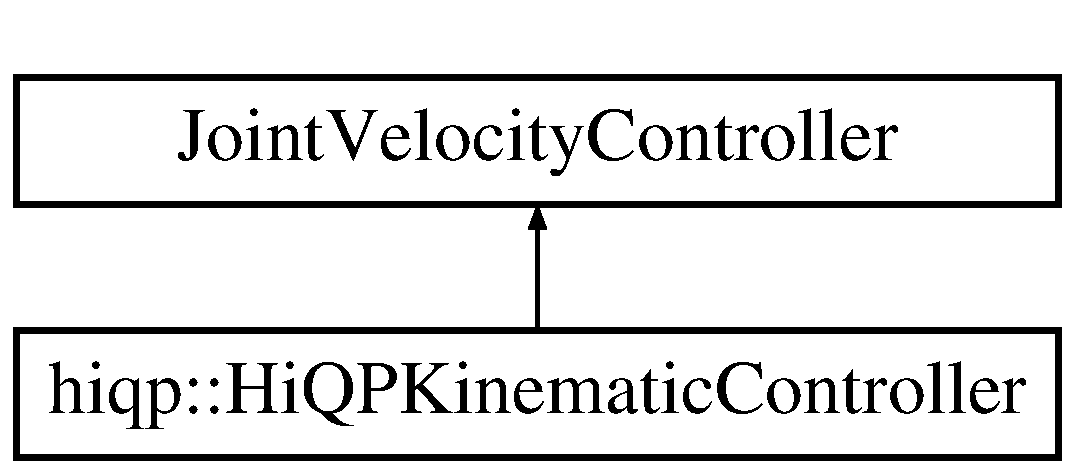
\includegraphics[height=2.000000cm]{classhiqp_1_1HiQPKinematicController}
\end{center}
\end{figure}
\subsection*{Public Member Functions}
\begin{DoxyCompactItemize}
\item 
\hypertarget{classhiqp_1_1HiQPKinematicController_a3dd9c3d69dc2a4beafe67b1b5ac2de50}{\hyperlink{classhiqp_1_1HiQPKinematicController_a3dd9c3d69dc2a4beafe67b1b5ac2de50}{Hi\-Q\-P\-Kinematic\-Controller} ()}\label{classhiqp_1_1HiQPKinematicController_a3dd9c3d69dc2a4beafe67b1b5ac2de50}

\begin{DoxyCompactList}\small\item\em Constructor Constructs my awesome controller. \end{DoxyCompactList}\item 
\hypertarget{classhiqp_1_1HiQPKinematicController_a4d99b3f5ef8059e22c4826726ebc3327}{\hyperlink{classhiqp_1_1HiQPKinematicController_a4d99b3f5ef8059e22c4826726ebc3327}{$\sim$\-Hi\-Q\-P\-Kinematic\-Controller} () noexcept}\label{classhiqp_1_1HiQPKinematicController_a4d99b3f5ef8059e22c4826726ebc3327}

\begin{DoxyCompactList}\small\item\em Destructor Destructs my awesome controller \-:(. \end{DoxyCompactList}\item 
bool \hyperlink{classhiqp_1_1HiQPKinematicController_a3aa91fd2992e5b0647a34fe61c97d23f}{init} (\hyperlink{namespacehiqp_ac536ca3b4ba33489281fa5bec490799c}{Joint\-Velocity\-Interface} $\ast$hw, ros\-::\-Node\-Handle \&controller\-\_\-nh)
\begin{DoxyCompactList}\small\item\em Called every time the controller is initialized by the ros\-::controller\-\_\-manager. \end{DoxyCompactList}\item 
void \hyperlink{classhiqp_1_1HiQPKinematicController_ad7b0146f120356c6ed350ff8ed7760d5}{starting} (const ros\-::\-Time \&time)
\begin{DoxyCompactList}\small\item\em Called every time the controller is started by the ros\-::controller\-\_\-manager. \end{DoxyCompactList}\item 
void \hyperlink{classhiqp_1_1HiQPKinematicController_abec4762d2aaac2bcdac7b0e135e68d48}{update} (const ros\-::\-Time \&time, const ros\-::\-Duration \&period)
\begin{DoxyCompactList}\small\item\em Called every time the controller is updated by the ros\-::controller\-\_\-manager. \end{DoxyCompactList}\item 
void \hyperlink{classhiqp_1_1HiQPKinematicController_ad23d401ef3f80bfc3a1af5f078f8b7f8}{stopping} (const ros\-::\-Time \&time)
\begin{DoxyCompactList}\small\item\em Called every time the controller is stopped by the ros\-::controller\-\_\-manager. \end{DoxyCompactList}\end{DoxyCompactItemize}


\subsection{Detailed Description}
This is my awesome controller. 

It's awesome! 

\subsection{Member Function Documentation}
\hypertarget{classhiqp_1_1HiQPKinematicController_a3aa91fd2992e5b0647a34fe61c97d23f}{\index{hiqp\-::\-Hi\-Q\-P\-Kinematic\-Controller@{hiqp\-::\-Hi\-Q\-P\-Kinematic\-Controller}!init@{init}}
\index{init@{init}!hiqp::HiQPKinematicController@{hiqp\-::\-Hi\-Q\-P\-Kinematic\-Controller}}
\subsubsection[{init}]{\setlength{\rightskip}{0pt plus 5cm}bool hiqp\-::\-Hi\-Q\-P\-Kinematic\-Controller\-::init (
\begin{DoxyParamCaption}
\item[{{\bf Joint\-Velocity\-Interface} $\ast$}]{hw, }
\item[{ros\-::\-Node\-Handle \&}]{controller\-\_\-nh}
\end{DoxyParamCaption}
)}}\label{classhiqp_1_1HiQPKinematicController_a3aa91fd2992e5b0647a34fe61c97d23f}


Called every time the controller is initialized by the ros\-::controller\-\_\-manager. 

Does some cool stuff!


\begin{DoxyParams}{Parameters}
{\em hw} & \-: a pointer to the hardware interface used by this controller \\
\hline
{\em controller\-\_\-nh} & \-: the node handle of this controller \\
\hline
\end{DoxyParams}
\begin{DoxyReturn}{Returns}
true if the initialization was successful 
\end{DoxyReturn}
\hypertarget{classhiqp_1_1HiQPKinematicController_ad7b0146f120356c6ed350ff8ed7760d5}{\index{hiqp\-::\-Hi\-Q\-P\-Kinematic\-Controller@{hiqp\-::\-Hi\-Q\-P\-Kinematic\-Controller}!starting@{starting}}
\index{starting@{starting}!hiqp::HiQPKinematicController@{hiqp\-::\-Hi\-Q\-P\-Kinematic\-Controller}}
\subsubsection[{starting}]{\setlength{\rightskip}{0pt plus 5cm}void hiqp\-::\-Hi\-Q\-P\-Kinematic\-Controller\-::starting (
\begin{DoxyParamCaption}
\item[{const ros\-::\-Time \&}]{time}
\end{DoxyParamCaption}
)}}\label{classhiqp_1_1HiQPKinematicController_ad7b0146f120356c6ed350ff8ed7760d5}


Called every time the controller is started by the ros\-::controller\-\_\-manager. 

Does some cool stuff!


\begin{DoxyParams}{Parameters}
{\em time} & \-: the current wall-\/time in R\-O\-S \\
\hline
\end{DoxyParams}
\begin{DoxyReturn}{Returns}
true if the starting was successful 
\end{DoxyReturn}
\hypertarget{classhiqp_1_1HiQPKinematicController_ad23d401ef3f80bfc3a1af5f078f8b7f8}{\index{hiqp\-::\-Hi\-Q\-P\-Kinematic\-Controller@{hiqp\-::\-Hi\-Q\-P\-Kinematic\-Controller}!stopping@{stopping}}
\index{stopping@{stopping}!hiqp::HiQPKinematicController@{hiqp\-::\-Hi\-Q\-P\-Kinematic\-Controller}}
\subsubsection[{stopping}]{\setlength{\rightskip}{0pt plus 5cm}void hiqp\-::\-Hi\-Q\-P\-Kinematic\-Controller\-::stopping (
\begin{DoxyParamCaption}
\item[{const ros\-::\-Time \&}]{time}
\end{DoxyParamCaption}
)}}\label{classhiqp_1_1HiQPKinematicController_ad23d401ef3f80bfc3a1af5f078f8b7f8}


Called every time the controller is stopped by the ros\-::controller\-\_\-manager. 

Does some cool stuff!


\begin{DoxyParams}{Parameters}
{\em time} & \-: the current wall-\/time in R\-O\-S \\
\hline
\end{DoxyParams}
\begin{DoxyReturn}{Returns}
true if the stopping was successful 
\end{DoxyReturn}
\hypertarget{classhiqp_1_1HiQPKinematicController_abec4762d2aaac2bcdac7b0e135e68d48}{\index{hiqp\-::\-Hi\-Q\-P\-Kinematic\-Controller@{hiqp\-::\-Hi\-Q\-P\-Kinematic\-Controller}!update@{update}}
\index{update@{update}!hiqp::HiQPKinematicController@{hiqp\-::\-Hi\-Q\-P\-Kinematic\-Controller}}
\subsubsection[{update}]{\setlength{\rightskip}{0pt plus 5cm}void hiqp\-::\-Hi\-Q\-P\-Kinematic\-Controller\-::update (
\begin{DoxyParamCaption}
\item[{const ros\-::\-Time \&}]{time, }
\item[{const ros\-::\-Duration \&}]{period}
\end{DoxyParamCaption}
)}}\label{classhiqp_1_1HiQPKinematicController_abec4762d2aaac2bcdac7b0e135e68d48}


Called every time the controller is updated by the ros\-::controller\-\_\-manager. 

The function\-: 
\begin{DoxyEnumerate}
\item locks a mutex and reads position and velocity values from the joint handles, 
\item calls get\-Kinematic\-Controls() on its task manager, 
\item and locks a mutex and writes velocity values to the joint handles. 
\end{DoxyEnumerate}The joint handles are stored as a map between the joints q-\/number in the K\-D\-L\-::\-Tree and the joint handles themselves.


\begin{DoxyParams}{Parameters}
{\em time} & \-: the current wall-\/time in R\-O\-S \\
\hline
{\em period} & \-: the time between the last update call and this, i.\-e. the sample time. \\
\hline
\end{DoxyParams}
\begin{DoxyReturn}{Returns}
true if the update was successful 
\end{DoxyReturn}


The documentation for this class was generated from the following files\-:\begin{DoxyCompactItemize}
\item 
include/hiqp/\hyperlink{hiqp__kinematic__controller_8h}{hiqp\-\_\-kinematic\-\_\-controller.\-h}\item 
src/\hyperlink{hiqp__kinematic__controller_8cpp}{hiqp\-\_\-kinematic\-\_\-controller.\-cpp}\end{DoxyCompactItemize}

\hypertarget{classhiqp_1_1Task}{\section{hiqp\-:\-:Task Class Reference}
\label{classhiqp_1_1Task}\index{hiqp\-::\-Task@{hiqp\-::\-Task}}
}
Inheritance diagram for hiqp\-:\-:Task\-:\begin{figure}[H]
\begin{center}
\leavevmode
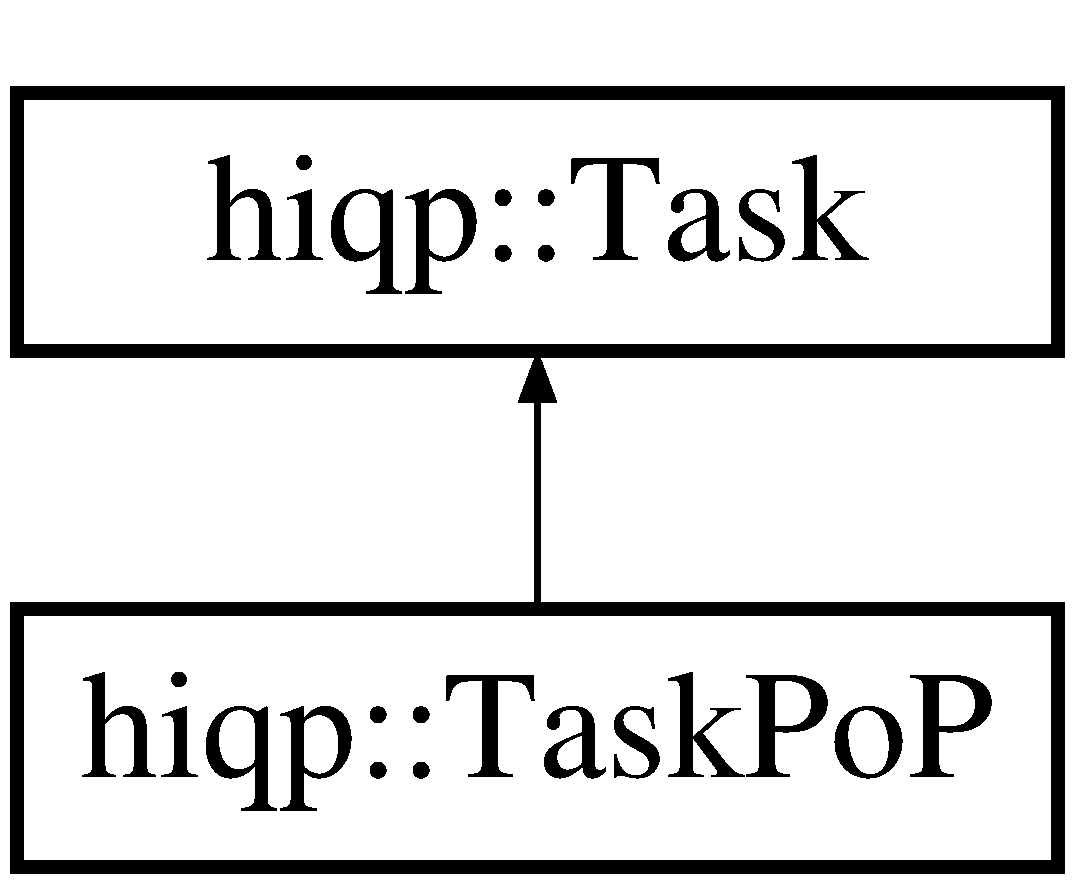
\includegraphics[height=2.000000cm]{classhiqp_1_1Task}
\end{center}
\end{figure}
\subsection*{Public Member Functions}
\begin{DoxyCompactItemize}
\item 
\hypertarget{classhiqp_1_1Task_a556692dacc6abb51d0437f59594026d9}{\hyperlink{classhiqp_1_1Task_a556692dacc6abb51d0437f59594026d9}{Task} ()}\label{classhiqp_1_1Task_a556692dacc6abb51d0437f59594026d9}

\begin{DoxyCompactList}\small\item\em Constructor Constructs my awesome task. \end{DoxyCompactList}\item 
\hypertarget{classhiqp_1_1Task_a73b4e41812713f28557c8d15925587db}{\hyperlink{classhiqp_1_1Task_a73b4e41812713f28557c8d15925587db}{$\sim$\-Task} () noexcept}\label{classhiqp_1_1Task_a73b4e41812713f28557c8d15925587db}

\begin{DoxyCompactList}\small\item\em Destructor Destructs my awesome task. \end{DoxyCompactList}\item 
\hypertarget{classhiqp_1_1Task_a02b6ccead41f86f26e7d1b2cb2e013ae}{virtual int {\bfseries init} (const std\-::vector$<$ std\-::string $>$ \&parameters)=0}\label{classhiqp_1_1Task_a02b6ccead41f86f26e7d1b2cb2e013ae}

\item 
virtual int \hyperlink{classhiqp_1_1Task_a2f81c249b39a1fd6557501d61548917b}{apply} (const K\-D\-L\-::\-Tree \&kdl\-\_\-tree, const K\-D\-L\-::\-Jnt\-Array\-Vel \&kdl\-\_\-joint\-\_\-pos\-\_\-vel)=0
\begin{DoxyCompactList}\small\item\em {\itshape Pure virtual}. Calculates the task function and task jacobian values. \end{DoxyCompactList}\item 
\hypertarget{classhiqp_1_1Task_a0d018a8a797cb730111614a9230d59e2}{virtual int {\bfseries draw} ()=0}\label{classhiqp_1_1Task_a0d018a8a797cb730111614a9230d59e2}

\end{DoxyCompactItemize}
\subsection*{Protected Member Functions}
\begin{DoxyCompactItemize}
\item 
\hypertarget{classhiqp_1_1Task_adbd4a69acbd2402d14fc51446d9c7a94}{\hyperlink{classhiqp_1_1TaskVisualizer}{Task\-Visualizer} $\ast$ {\bfseries get\-Task\-Visualizer} ()}\label{classhiqp_1_1Task_adbd4a69acbd2402d14fc51446d9c7a94}

\end{DoxyCompactItemize}
\subsection*{Protected Attributes}
\begin{DoxyCompactItemize}
\item 
\hypertarget{classhiqp_1_1Task_af1290bb9764f71d8abd3c26eb6997425}{double {\bfseries e\-\_\-}}\label{classhiqp_1_1Task_af1290bb9764f71d8abd3c26eb6997425}

\item 
\hypertarget{classhiqp_1_1Task_a10cc3261be638fbc5778c1ee71c16784}{Eigen\-::\-Matrix\-Xd {\bfseries J\-\_\-}}\label{classhiqp_1_1Task_a10cc3261be638fbc5778c1ee71c16784}

\end{DoxyCompactItemize}


\subsection{Member Function Documentation}
\hypertarget{classhiqp_1_1Task_a2f81c249b39a1fd6557501d61548917b}{\index{hiqp\-::\-Task@{hiqp\-::\-Task}!apply@{apply}}
\index{apply@{apply}!hiqp::Task@{hiqp\-::\-Task}}
\subsubsection[{apply}]{\setlength{\rightskip}{0pt plus 5cm}virtual int hiqp\-::\-Task\-::apply (
\begin{DoxyParamCaption}
\item[{const K\-D\-L\-::\-Tree \&}]{kdl\-\_\-tree, }
\item[{const K\-D\-L\-::\-Jnt\-Array\-Vel \&}]{kdl\-\_\-joint\-\_\-pos\-\_\-vel}
\end{DoxyParamCaption}
)\hspace{0.3cm}{\ttfamily [pure virtual]}}}\label{classhiqp_1_1Task_a2f81c249b39a1fd6557501d61548917b}


{\itshape Pure virtual}. Calculates the task function and task jacobian values. 


\begin{DoxyParams}{Parameters}
{\em kdl\-\_\-tree} & \-: reference to the kinematic dynamic tree of the robot \\
\hline
{\em kdl\-\_\-joint\-\_\-pos\-\_\-vel} & \-: reference to the current joint positions and velocities \\
\hline
{\em task\-\_\-fun\-\_\-val} & \-: reference to where the output controls are to be stored\\
\hline
\end{DoxyParams}
\begin{DoxyReturn}{Returns}
0 if the calculation was successful 
\end{DoxyReturn}


Implemented in \hyperlink{classhiqp_1_1TaskPoP_a7f50f65c7e09492a0021715ad2ef2866}{hiqp\-::\-Task\-Po\-P}.



The documentation for this class was generated from the following file\-:\begin{DoxyCompactItemize}
\item 
include/hiqp/\hyperlink{task_8h}{task.\-h}\end{DoxyCompactItemize}

\hypertarget{classhiqp_1_1TaskBehaviour}{\section{hiqp\-:\-:Task\-Behaviour Class Reference}
\label{classhiqp_1_1TaskBehaviour}\index{hiqp\-::\-Task\-Behaviour@{hiqp\-::\-Task\-Behaviour}}
}
Inheritance diagram for hiqp\-:\-:Task\-Behaviour\-:\begin{figure}[H]
\begin{center}
\leavevmode
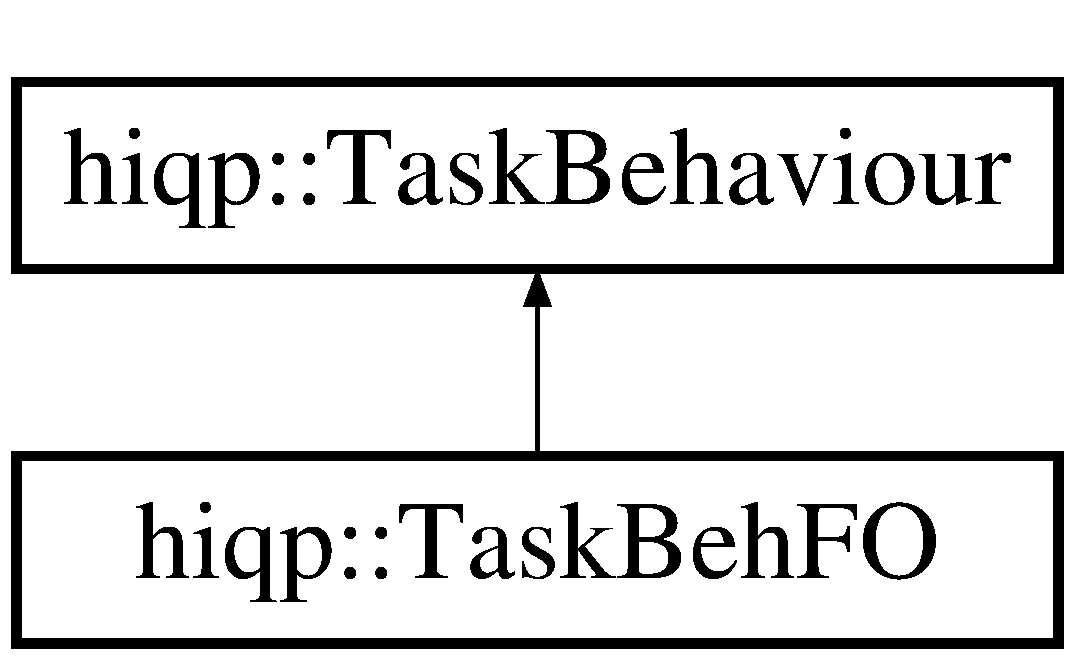
\includegraphics[height=2.000000cm]{classhiqp_1_1TaskBehaviour}
\end{center}
\end{figure}
\subsection*{Public Member Functions}
\begin{DoxyCompactItemize}
\item 
\hypertarget{classhiqp_1_1TaskBehaviour_acffdda2b407d55672ed9c7cb78c663ae}{virtual int {\bfseries init} (const std\-::vector$<$ std\-::string $>$ \&parameters)=0}\label{classhiqp_1_1TaskBehaviour_acffdda2b407d55672ed9c7cb78c663ae}

\item 
\hypertarget{classhiqp_1_1TaskBehaviour_aac31dd97622dfe8ed812f44c2e9d5d1e}{virtual int {\bfseries apply} (double e, const Eigen\-::\-Matrix\-Xd \&J, std\-::vector$<$ double $>$ \&controls)=0}\label{classhiqp_1_1TaskBehaviour_aac31dd97622dfe8ed812f44c2e9d5d1e}

\end{DoxyCompactItemize}


The documentation for this class was generated from the following file\-:\begin{DoxyCompactItemize}
\item 
include/hiqp/\hyperlink{task__behaviour_8h}{task\-\_\-behaviour.\-h}\end{DoxyCompactItemize}

\hypertarget{classhiqp_1_1TaskBehFO}{\section{hiqp\-:\-:Task\-Beh\-F\-O Class Reference}
\label{classhiqp_1_1TaskBehFO}\index{hiqp\-::\-Task\-Beh\-F\-O@{hiqp\-::\-Task\-Beh\-F\-O}}
}
Inheritance diagram for hiqp\-:\-:Task\-Beh\-F\-O\-:\begin{figure}[H]
\begin{center}
\leavevmode
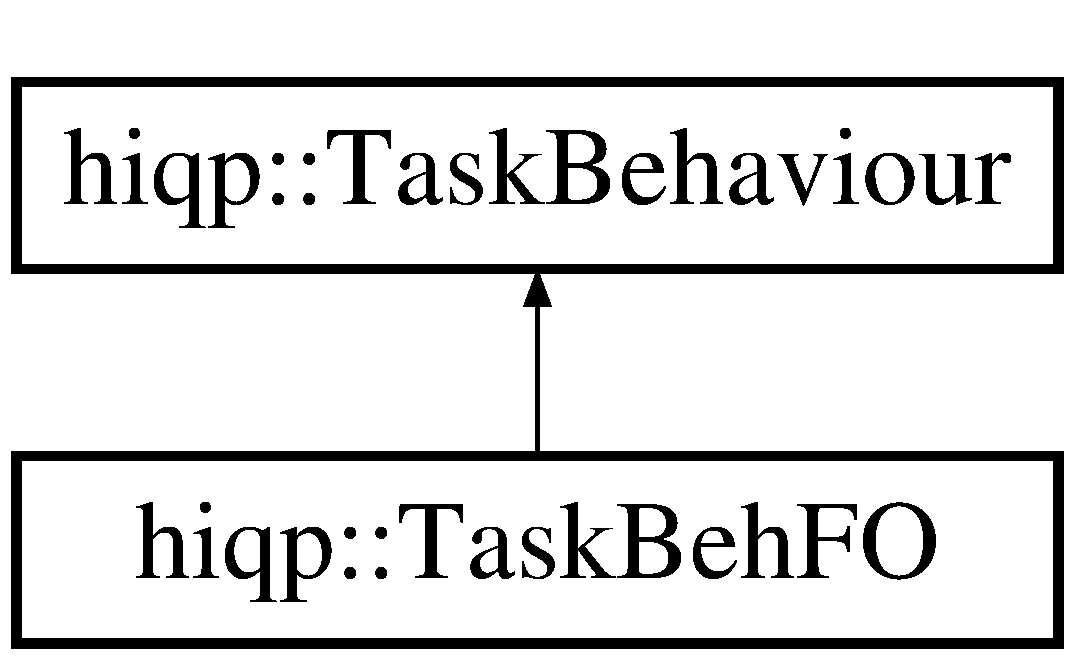
\includegraphics[height=2.000000cm]{classhiqp_1_1TaskBehFO}
\end{center}
\end{figure}
\subsection*{Public Member Functions}
\begin{DoxyCompactItemize}
\item 
\hypertarget{classhiqp_1_1TaskBehFO_a9eaee2261d1854b355d414e8392286e6}{int {\bfseries init} (const std\-::vector$<$ std\-::string $>$ \&parameters)}\label{classhiqp_1_1TaskBehFO_a9eaee2261d1854b355d414e8392286e6}

\item 
\hypertarget{classhiqp_1_1TaskBehFO_abe51a68d08d4a6886cca42e52d0c2fe8}{int {\bfseries apply} (double e, const Eigen\-::\-Matrix\-Xd \&J, std\-::vector$<$ double $>$ \&controls)}\label{classhiqp_1_1TaskBehFO_abe51a68d08d4a6886cca42e52d0c2fe8}

\end{DoxyCompactItemize}


The documentation for this class was generated from the following files\-:\begin{DoxyCompactItemize}
\item 
include/hiqp/\hyperlink{task__beh__fo_8h}{task\-\_\-beh\-\_\-fo.\-h}\item 
src/\hyperlink{task__beh__fo_8cpp}{task\-\_\-beh\-\_\-fo.\-cpp}\end{DoxyCompactItemize}

\hypertarget{classhiqp_1_1TaskManager}{\section{hiqp\-:\-:Task\-Manager Class Reference}
\label{classhiqp_1_1TaskManager}\index{hiqp\-::\-Task\-Manager@{hiqp\-::\-Task\-Manager}}
}


Should be created only once!  




{\ttfamily \#include $<$task\-\_\-manager.\-h$>$}

\subsection*{Public Member Functions}
\begin{DoxyCompactItemize}
\item 
\hypertarget{classhiqp_1_1TaskManager_af190d8f0b3ee1c0d32acdb70fae6e03d}{\hyperlink{classhiqp_1_1TaskManager_af190d8f0b3ee1c0d32acdb70fae6e03d}{Task\-Manager} ()}\label{classhiqp_1_1TaskManager_af190d8f0b3ee1c0d32acdb70fae6e03d}

\begin{DoxyCompactList}\small\item\em Constructor Constructs my awesome controller. \end{DoxyCompactList}\item 
\hypertarget{classhiqp_1_1TaskManager_a688ad548e2ef681b458c1fc90326f6e6}{\hyperlink{classhiqp_1_1TaskManager_a688ad548e2ef681b458c1fc90326f6e6}{$\sim$\-Task\-Manager} () noexcept}\label{classhiqp_1_1TaskManager_a688ad548e2ef681b458c1fc90326f6e6}

\begin{DoxyCompactList}\small\item\em Destructor Destructs my awesome manager. \end{DoxyCompactList}\item 
bool \hyperlink{classhiqp_1_1TaskManager_a9243435c3819b03a9874f47d985a2147}{get\-Kinematic\-Controls} (const K\-D\-L\-::\-Tree \&kdl\-\_\-tree, const K\-D\-L\-::\-Jnt\-Array\-Vel \&kdl\-\_\-joint\-\_\-pos\-\_\-vel, unsigned int n\-\_\-controls, std\-::vector$<$ double $>$ \&controls)
\begin{DoxyCompactList}\small\item\em Called every time the controller is initialized by the ros\-::controller\-\_\-manager. \end{DoxyCompactList}\end{DoxyCompactItemize}


\subsection{Detailed Description}
Should be created only once! 

It's awesome! 

\subsection{Member Function Documentation}
\hypertarget{classhiqp_1_1TaskManager_a9243435c3819b03a9874f47d985a2147}{\index{hiqp\-::\-Task\-Manager@{hiqp\-::\-Task\-Manager}!get\-Kinematic\-Controls@{get\-Kinematic\-Controls}}
\index{get\-Kinematic\-Controls@{get\-Kinematic\-Controls}!hiqp::TaskManager@{hiqp\-::\-Task\-Manager}}
\subsubsection[{get\-Kinematic\-Controls}]{\setlength{\rightskip}{0pt plus 5cm}bool hiqp\-::\-Task\-Manager\-::get\-Kinematic\-Controls (
\begin{DoxyParamCaption}
\item[{const K\-D\-L\-::\-Tree \&}]{kdl\-\_\-tree, }
\item[{const K\-D\-L\-::\-Jnt\-Array\-Vel \&}]{kdl\-\_\-joint\-\_\-pos\-\_\-vel, }
\item[{unsigned int}]{n\-\_\-controls, }
\item[{std\-::vector$<$ double $>$ \&}]{controls}
\end{DoxyParamCaption}
)}}\label{classhiqp_1_1TaskManager_a9243435c3819b03a9874f47d985a2147}


Called every time the controller is initialized by the ros\-::controller\-\_\-manager. 

Does some cool stuff!


\begin{DoxyParams}{Parameters}
{\em kdl\-\_\-tree} & \-: the kinematic dynamic tree of the robot \\
\hline
{\em n\-\_\-controls} & \-: the number of controls \\
\hline
{\em controls} & \-: reference to the controls data \\
\hline
\end{DoxyParams}
\begin{DoxyReturn}{Returns}
true if the initialization was successful 
\end{DoxyReturn}


The documentation for this class was generated from the following files\-:\begin{DoxyCompactItemize}
\item 
include/\hyperlink{task__manager_8h}{task\-\_\-manager.\-h}\item 
src/task\-\_\-manager.\-cpp\end{DoxyCompactItemize}

\hypertarget{classhiqp_1_1TaskPoP}{\section{hiqp\-:\-:Task\-Po\-P Class Reference}
\label{classhiqp_1_1TaskPoP}\index{hiqp\-::\-Task\-Po\-P@{hiqp\-::\-Task\-Po\-P}}
}
Inheritance diagram for hiqp\-:\-:Task\-Po\-P\-:\begin{figure}[H]
\begin{center}
\leavevmode
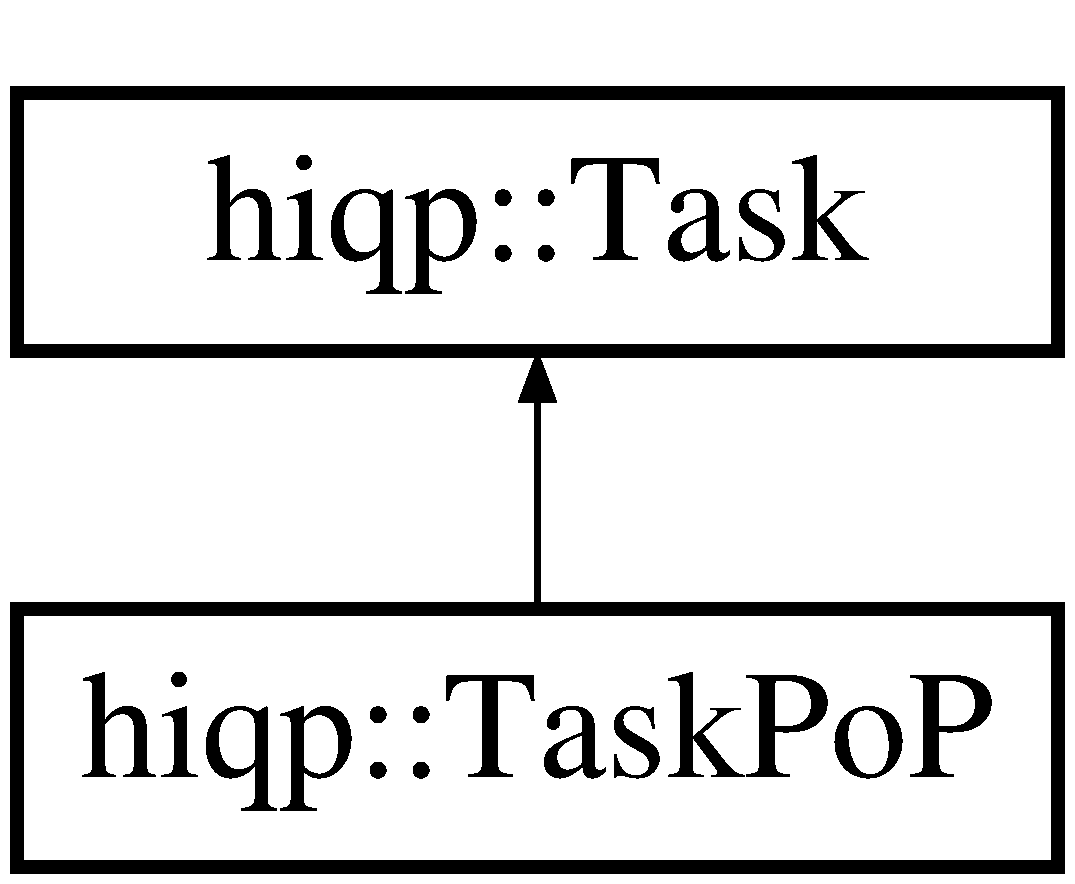
\includegraphics[height=2.000000cm]{classhiqp_1_1TaskPoP}
\end{center}
\end{figure}
\subsection*{Public Member Functions}
\begin{DoxyCompactItemize}
\item 
\hypertarget{classhiqp_1_1TaskPoP_a0d7d964d7cd4421897d7eaf1c16dfce9}{\hyperlink{classhiqp_1_1TaskPoP_a0d7d964d7cd4421897d7eaf1c16dfce9}{Task\-Po\-P} ()}\label{classhiqp_1_1TaskPoP_a0d7d964d7cd4421897d7eaf1c16dfce9}

\begin{DoxyCompactList}\small\item\em Constructor Constructs my awesome task. \end{DoxyCompactList}\item 
\hypertarget{classhiqp_1_1TaskPoP_ae8409bea63d95e02bd740e6aaa70b4fe}{\hyperlink{classhiqp_1_1TaskPoP_ae8409bea63d95e02bd740e6aaa70b4fe}{$\sim$\-Task\-Po\-P} () noexcept}\label{classhiqp_1_1TaskPoP_ae8409bea63d95e02bd740e6aaa70b4fe}

\begin{DoxyCompactList}\small\item\em Destructor Destructs my awesome task. \end{DoxyCompactList}\item 
int \hyperlink{classhiqp_1_1TaskPoP_a23279792f72d60c49a941be747d5a641}{init} (const std\-::vector$<$ std\-::string $>$ \&parameters)
\begin{DoxyCompactList}\small\item\em {\itshape Pure virtual}. Initializes the task \end{DoxyCompactList}\item 
int \hyperlink{classhiqp_1_1TaskPoP_a7f50f65c7e09492a0021715ad2ef2866}{apply} (const K\-D\-L\-::\-Tree \&kdl\-\_\-tree, const K\-D\-L\-::\-Jnt\-Array\-Vel \&kdl\-\_\-joint\-\_\-pos\-\_\-vel)
\begin{DoxyCompactList}\small\item\em {\itshape Pure virtual}. Calculates the task function and task jacobian values. \end{DoxyCompactList}\item 
int \hyperlink{classhiqp_1_1TaskPoP_a5e7a17a2371c5a3d28986c4cb4c09319}{draw} ()
\begin{DoxyCompactList}\small\item\em {\itshape Pure virtual}. Draws the task \end{DoxyCompactList}\end{DoxyCompactItemize}
\subsection*{Additional Inherited Members}


\subsection{Member Function Documentation}
\hypertarget{classhiqp_1_1TaskPoP_a7f50f65c7e09492a0021715ad2ef2866}{\index{hiqp\-::\-Task\-Po\-P@{hiqp\-::\-Task\-Po\-P}!apply@{apply}}
\index{apply@{apply}!hiqp::TaskPoP@{hiqp\-::\-Task\-Po\-P}}
\subsubsection[{apply}]{\setlength{\rightskip}{0pt plus 5cm}int hiqp\-::\-Task\-Po\-P\-::apply (
\begin{DoxyParamCaption}
\item[{const K\-D\-L\-::\-Tree \&}]{kdl\-\_\-tree, }
\item[{const K\-D\-L\-::\-Jnt\-Array\-Vel \&}]{kdl\-\_\-joint\-\_\-pos\-\_\-vel}
\end{DoxyParamCaption}
)\hspace{0.3cm}{\ttfamily [virtual]}}}\label{classhiqp_1_1TaskPoP_a7f50f65c7e09492a0021715ad2ef2866}


{\itshape Pure virtual}. Calculates the task function and task jacobian values. 


\begin{DoxyParams}{Parameters}
{\em kdl\-\_\-tree} & \-: reference to the kinematic dynamic tree of the robot \\
\hline
{\em joints\-\_\-pos\-\_\-vel} & \-: reference to the current joint positions and velocities\\
\hline
\end{DoxyParams}
\begin{DoxyReturn}{Returns}
true if the calculation was successful 
\end{DoxyReturn}


Implements \hyperlink{classhiqp_1_1Task_a2f81c249b39a1fd6557501d61548917b}{hiqp\-::\-Task}.

\hypertarget{classhiqp_1_1TaskPoP_a5e7a17a2371c5a3d28986c4cb4c09319}{\index{hiqp\-::\-Task\-Po\-P@{hiqp\-::\-Task\-Po\-P}!draw@{draw}}
\index{draw@{draw}!hiqp::TaskPoP@{hiqp\-::\-Task\-Po\-P}}
\subsubsection[{draw}]{\setlength{\rightskip}{0pt plus 5cm}int hiqp\-::\-Task\-Po\-P\-::draw (
\begin{DoxyParamCaption}
{}
\end{DoxyParamCaption}
)\hspace{0.3cm}{\ttfamily [virtual]}}}\label{classhiqp_1_1TaskPoP_a5e7a17a2371c5a3d28986c4cb4c09319}


{\itshape Pure virtual}. Draws the task 

\begin{DoxyReturn}{Returns}
0 upon success 
\end{DoxyReturn}


Implements \hyperlink{classhiqp_1_1Task}{hiqp\-::\-Task}.

\hypertarget{classhiqp_1_1TaskPoP_a23279792f72d60c49a941be747d5a641}{\index{hiqp\-::\-Task\-Po\-P@{hiqp\-::\-Task\-Po\-P}!init@{init}}
\index{init@{init}!hiqp::TaskPoP@{hiqp\-::\-Task\-Po\-P}}
\subsubsection[{init}]{\setlength{\rightskip}{0pt plus 5cm}int hiqp\-::\-Task\-Po\-P\-::init (
\begin{DoxyParamCaption}
\item[{const std\-::vector$<$ std\-::string $>$ \&}]{parameters}
\end{DoxyParamCaption}
)\hspace{0.3cm}{\ttfamily [virtual]}}}\label{classhiqp_1_1TaskPoP_a23279792f72d60c49a941be747d5a641}


{\itshape Pure virtual}. Initializes the task 

\begin{DoxyReturn}{Returns}
0 upon success 
\end{DoxyReturn}


Implements \hyperlink{classhiqp_1_1Task}{hiqp\-::\-Task}.



The documentation for this class was generated from the following files\-:\begin{DoxyCompactItemize}
\item 
include/hiqp/\hyperlink{task__pop_8h}{task\-\_\-pop.\-h}\item 
src/\hyperlink{task__pop_8cpp}{task\-\_\-pop.\-cpp}\end{DoxyCompactItemize}

\hypertarget{classhiqp_1_1TaskVisualizer}{\section{hiqp\-:\-:Task\-Visualizer Class Reference}
\label{classhiqp_1_1TaskVisualizer}\index{hiqp\-::\-Task\-Visualizer@{hiqp\-::\-Task\-Visualizer}}
}
\subsection*{Public Member Functions}
\begin{DoxyCompactItemize}
\item 
\hypertarget{classhiqp_1_1TaskVisualizer_adbbab9f82514fe7ccd96e5c6e16be780}{int {\bfseries init} (ros\-::\-Node\-Handle $\ast$controller\-\_\-nh)}\label{classhiqp_1_1TaskVisualizer_adbbab9f82514fe7ccd96e5c6e16be780}

\item 
int \hyperlink{classhiqp_1_1TaskVisualizer_ac591685c77aa46472120dad1483cb7e1}{set\-Visibility} (std\-::size\-\_\-t id, bool visibility)
\begin{DoxyCompactList}\small\item\em Sets the visibility of the object (more efficient than setting alpha to zero) \end{DoxyCompactList}\item 
std\-::size\-\_\-t \hyperlink{classhiqp_1_1TaskVisualizer_a538bfbc2c33a5ed03feaedfc1ae06fac}{create\-Plane} (double nx, double ny, double nz, double d, double r, double g, double b, double a)
\begin{DoxyCompactList}\small\item\em Creates and registers a plane among the objects to be visualized. \end{DoxyCompactList}\item 
int \hyperlink{classhiqp_1_1TaskVisualizer_acac4eca22d5adadac5857327d06d9b5a}{set\-Plane\-Geometry} (std\-::size\-\_\-t id, double nx, double ny, double nz, double d)
\begin{DoxyCompactList}\small\item\em Sets an already existing planes geometry. \end{DoxyCompactList}\item 
int \hyperlink{classhiqp_1_1TaskVisualizer_a9615b534b49aa9d9cf0c2d91cd10ba0e}{set\-Plane\-Esthetics} (std\-::size\-\_\-t id, double r, double g, double b, double a)
\begin{DoxyCompactList}\small\item\em Sets an already existing planes esthetics. \end{DoxyCompactList}\end{DoxyCompactItemize}


\subsection{Member Function Documentation}
\hypertarget{classhiqp_1_1TaskVisualizer_a538bfbc2c33a5ed03feaedfc1ae06fac}{\index{hiqp\-::\-Task\-Visualizer@{hiqp\-::\-Task\-Visualizer}!create\-Plane@{create\-Plane}}
\index{create\-Plane@{create\-Plane}!hiqp::TaskVisualizer@{hiqp\-::\-Task\-Visualizer}}
\subsubsection[{create\-Plane}]{\setlength{\rightskip}{0pt plus 5cm}std\-::size\-\_\-t hiqp\-::\-Task\-Visualizer\-::create\-Plane (
\begin{DoxyParamCaption}
\item[{double}]{nx, }
\item[{double}]{ny, }
\item[{double}]{nz, }
\item[{double}]{d, }
\item[{double}]{r, }
\item[{double}]{g, }
\item[{double}]{b, }
\item[{double}]{a}
\end{DoxyParamCaption}
)}}\label{classhiqp_1_1TaskVisualizer_a538bfbc2c33a5ed03feaedfc1ae06fac}


Creates and registers a plane among the objects to be visualized. 


\begin{DoxyParams}{Parameters}
{\em nx} & \-: x-\/component of the normal vector of the plane \\
\hline
{\em ny} & \-: y-\/component of the normal vector of the plane \\
\hline
{\em nz} & \-: z-\/component of the normal vector of the plane \\
\hline
{\em d} & \-: distance from the plane to the origin \\
\hline
{\em red} & \-: the red color component (0-\/255) \\
\hline
{\em blue} & \-: the blue color component (0-\/255) \\
\hline
{\em green} & \-: the green color component (0-\/255) \\
\hline
{\em alpha} & \-: the alpha component (0-\/255)\\
\hline
\end{DoxyParams}
\begin{DoxyReturn}{Returns}
the unique identifier of the created task 
\end{DoxyReturn}
\hypertarget{classhiqp_1_1TaskVisualizer_a9615b534b49aa9d9cf0c2d91cd10ba0e}{\index{hiqp\-::\-Task\-Visualizer@{hiqp\-::\-Task\-Visualizer}!set\-Plane\-Esthetics@{set\-Plane\-Esthetics}}
\index{set\-Plane\-Esthetics@{set\-Plane\-Esthetics}!hiqp::TaskVisualizer@{hiqp\-::\-Task\-Visualizer}}
\subsubsection[{set\-Plane\-Esthetics}]{\setlength{\rightskip}{0pt plus 5cm}int hiqp\-::\-Task\-Visualizer\-::set\-Plane\-Esthetics (
\begin{DoxyParamCaption}
\item[{std\-::size\-\_\-t}]{id, }
\item[{double}]{r, }
\item[{double}]{g, }
\item[{double}]{b, }
\item[{double}]{a}
\end{DoxyParamCaption}
)}}\label{classhiqp_1_1TaskVisualizer_a9615b534b49aa9d9cf0c2d91cd10ba0e}


Sets an already existing planes esthetics. 


\begin{DoxyParams}{Parameters}
{\em id} & \-: the unique identifier of the plane \\
\hline
{\em red} & \-: the new red color component (0-\/255) \\
\hline
{\em blue} & \-: the new blue color component (0-\/255) \\
\hline
{\em green} & \-: the new green color component (0-\/255) \\
\hline
{\em alpha} & \-: the new alpha component (0-\/255)\\
\hline
\end{DoxyParams}
\begin{DoxyReturn}{Returns}
0 on success, -\/1 if the identifier was not found, -\/2 if the identifier was not associated with a plane primitive. 
\end{DoxyReturn}
\hypertarget{classhiqp_1_1TaskVisualizer_acac4eca22d5adadac5857327d06d9b5a}{\index{hiqp\-::\-Task\-Visualizer@{hiqp\-::\-Task\-Visualizer}!set\-Plane\-Geometry@{set\-Plane\-Geometry}}
\index{set\-Plane\-Geometry@{set\-Plane\-Geometry}!hiqp::TaskVisualizer@{hiqp\-::\-Task\-Visualizer}}
\subsubsection[{set\-Plane\-Geometry}]{\setlength{\rightskip}{0pt plus 5cm}int hiqp\-::\-Task\-Visualizer\-::set\-Plane\-Geometry (
\begin{DoxyParamCaption}
\item[{std\-::size\-\_\-t}]{id, }
\item[{double}]{nx, }
\item[{double}]{ny, }
\item[{double}]{nz, }
\item[{double}]{d}
\end{DoxyParamCaption}
)}}\label{classhiqp_1_1TaskVisualizer_acac4eca22d5adadac5857327d06d9b5a}


Sets an already existing planes geometry. 


\begin{DoxyParams}{Parameters}
{\em id} & \-: the unique identifier of the plane \\
\hline
{\em nx} & \-: the new x-\/component of the normal vector of the plane \\
\hline
{\em ny} & \-: the new y-\/component of the normal vector of the plane \\
\hline
{\em nz} & \-: the new z-\/component of the normal vector of the plane \\
\hline
{\em d} & \-: the new distance from the plane to the origin\\
\hline
\end{DoxyParams}
\begin{DoxyReturn}{Returns}
0 on success, -\/1 if the identifier was invalid 
\end{DoxyReturn}
\hypertarget{classhiqp_1_1TaskVisualizer_ac591685c77aa46472120dad1483cb7e1}{\index{hiqp\-::\-Task\-Visualizer@{hiqp\-::\-Task\-Visualizer}!set\-Visibility@{set\-Visibility}}
\index{set\-Visibility@{set\-Visibility}!hiqp::TaskVisualizer@{hiqp\-::\-Task\-Visualizer}}
\subsubsection[{set\-Visibility}]{\setlength{\rightskip}{0pt plus 5cm}int hiqp\-::\-Task\-Visualizer\-::set\-Visibility (
\begin{DoxyParamCaption}
\item[{std\-::size\-\_\-t}]{id, }
\item[{bool}]{visibility}
\end{DoxyParamCaption}
)}}\label{classhiqp_1_1TaskVisualizer_ac591685c77aa46472120dad1483cb7e1}


Sets the visibility of the object (more efficient than setting alpha to zero) 


\begin{DoxyParams}{Parameters}
{\em id} & \-: the identifier of the visual primitive \\
\hline
{\em visibility} & \-: the new visibility value\\
\hline
\end{DoxyParams}
\begin{DoxyReturn}{Returns}
0 on success, -\/1 if the primitive was not found 
\end{DoxyReturn}


The documentation for this class was generated from the following files\-:\begin{DoxyCompactItemize}
\item 
include/hiqp/\hyperlink{task__visualizer_8h}{task\-\_\-visualizer.\-h}\item 
src/\hyperlink{task__visualizer_8cpp}{task\-\_\-visualizer.\-cpp}\end{DoxyCompactItemize}

\hypertarget{classhiqp_1_1TaskVisualPlane}{\section{hiqp\-:\-:Task\-Visual\-Plane Class Reference}
\label{classhiqp_1_1TaskVisualPlane}\index{hiqp\-::\-Task\-Visual\-Plane@{hiqp\-::\-Task\-Visual\-Plane}}
}
Inheritance diagram for hiqp\-:\-:Task\-Visual\-Plane\-:\begin{figure}[H]
\begin{center}
\leavevmode
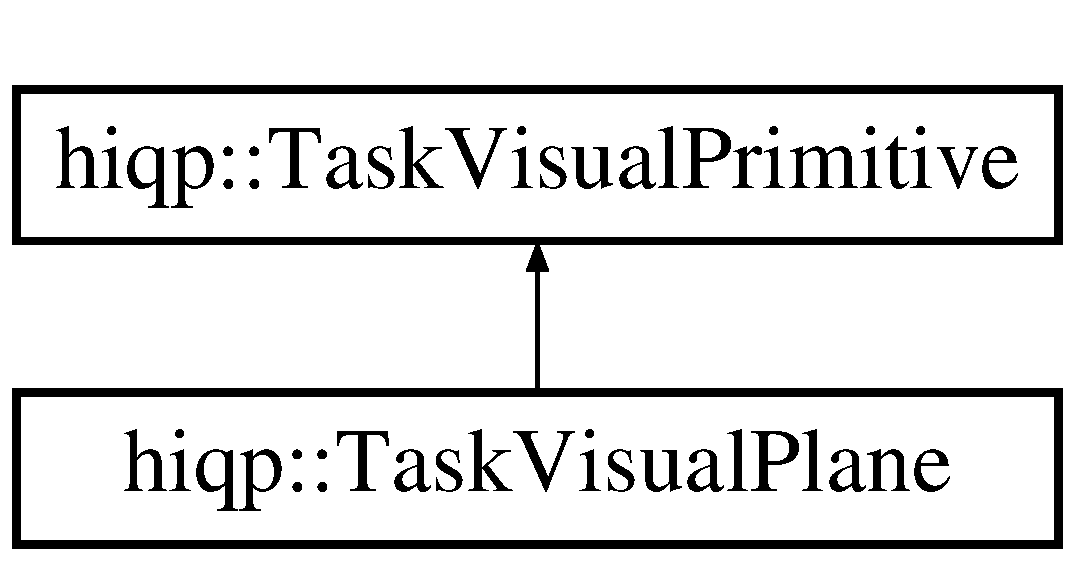
\includegraphics[height=2.000000cm]{classhiqp_1_1TaskVisualPlane}
\end{center}
\end{figure}
\subsection*{Public Member Functions}
\begin{DoxyCompactItemize}
\item 
\hypertarget{classhiqp_1_1TaskVisualPlane_a3c6cb31fd14a744949076f178533fd7b}{{\bfseries Task\-Visual\-Plane} (double nx, double ny, double nz, double d, double r, double g, double b, double a)}\label{classhiqp_1_1TaskVisualPlane_a3c6cb31fd14a744949076f178533fd7b}

\item 
\hypertarget{classhiqp_1_1TaskVisualPlane_aea03efd3dfaadc210644bdcae5437f7a}{void {\bfseries set\-Geometry} (double nx, double ny, double nz, double d)}\label{classhiqp_1_1TaskVisualPlane_aea03efd3dfaadc210644bdcae5437f7a}

\item 
\hypertarget{classhiqp_1_1TaskVisualPlane_a19969b5e40d92e0991f0d8997ce9550f}{void {\bfseries draw} (const ros\-::\-Publisher \&marker\-\_\-pub, int action)}\label{classhiqp_1_1TaskVisualPlane_a19969b5e40d92e0991f0d8997ce9550f}

\end{DoxyCompactItemize}
\subsection*{Public Attributes}
\begin{DoxyCompactItemize}
\item 
\hypertarget{classhiqp_1_1TaskVisualPlane_ab790d519f98ca0dd211ab0a1f2a189c5}{double {\bfseries nx\-\_\-}}\label{classhiqp_1_1TaskVisualPlane_ab790d519f98ca0dd211ab0a1f2a189c5}

\item 
\hypertarget{classhiqp_1_1TaskVisualPlane_a63abc244f4fcd197826878cc684c8557}{double {\bfseries ny\-\_\-}}\label{classhiqp_1_1TaskVisualPlane_a63abc244f4fcd197826878cc684c8557}

\item 
\hypertarget{classhiqp_1_1TaskVisualPlane_a4970d47a59369760c6768b6974d3f485}{double {\bfseries nz\-\_\-}}\label{classhiqp_1_1TaskVisualPlane_a4970d47a59369760c6768b6974d3f485}

\item 
\hypertarget{classhiqp_1_1TaskVisualPlane_a427c06f4ef32e4c2551cf3ea97fa029e}{double {\bfseries d\-\_\-}}\label{classhiqp_1_1TaskVisualPlane_a427c06f4ef32e4c2551cf3ea97fa029e}

\end{DoxyCompactItemize}


The documentation for this class was generated from the following file\-:\begin{DoxyCompactItemize}
\item 
src/\hyperlink{task__visualizer_8cpp}{task\-\_\-visualizer.\-cpp}\end{DoxyCompactItemize}

\hypertarget{classhiqp_1_1TaskVisualPrimitive}{\section{hiqp\-:\-:Task\-Visual\-Primitive Class Reference}
\label{classhiqp_1_1TaskVisualPrimitive}\index{hiqp\-::\-Task\-Visual\-Primitive@{hiqp\-::\-Task\-Visual\-Primitive}}
}
Inheritance diagram for hiqp\-:\-:Task\-Visual\-Primitive\-:\begin{figure}[H]
\begin{center}
\leavevmode
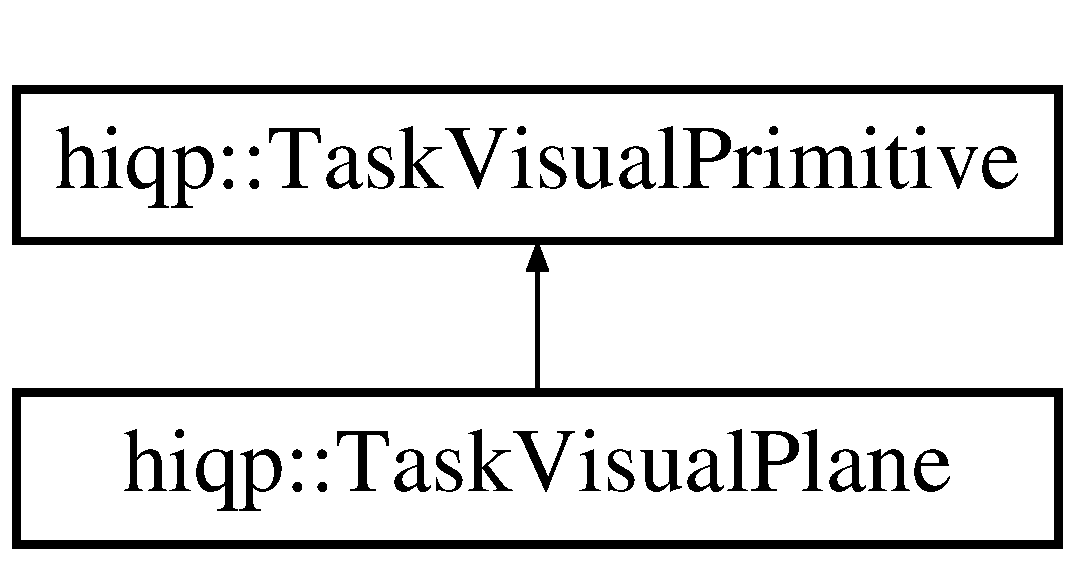
\includegraphics[height=2.000000cm]{classhiqp_1_1TaskVisualPrimitive}
\end{center}
\end{figure}
\subsection*{Public Member Functions}
\begin{DoxyCompactItemize}
\item 
\hypertarget{classhiqp_1_1TaskVisualPrimitive_afcac49ed0167f82760257b1193304f8c}{{\bfseries Task\-Visual\-Primitive} (double r, double g, double b, double a)}\label{classhiqp_1_1TaskVisualPrimitive_afcac49ed0167f82760257b1193304f8c}

\item 
\hypertarget{classhiqp_1_1TaskVisualPrimitive_add4cea0368114081cc191f072ae14971}{void {\bfseries set\-Esthetics} (double r, double g, double b, double a)}\label{classhiqp_1_1TaskVisualPrimitive_add4cea0368114081cc191f072ae14971}

\item 
\hypertarget{classhiqp_1_1TaskVisualPrimitive_a846fb1bd3c6ce220e9e53c35f6fac2de}{virtual void {\bfseries draw} (const ros\-::\-Publisher \&marker\-\_\-pub, int action)=0}\label{classhiqp_1_1TaskVisualPrimitive_a846fb1bd3c6ce220e9e53c35f6fac2de}

\end{DoxyCompactItemize}
\subsection*{Public Attributes}
\begin{DoxyCompactItemize}
\item 
\hypertarget{classhiqp_1_1TaskVisualPrimitive_ad09a580c9d583a967dda582ceb36a958}{std\-::size\-\_\-t {\bfseries id\-\_\-}}\label{classhiqp_1_1TaskVisualPrimitive_ad09a580c9d583a967dda582ceb36a958}

\item 
\hypertarget{classhiqp_1_1TaskVisualPrimitive_ad7baded10fdad47d75c698f3c05ab5b2}{bool {\bfseries visibility\-\_\-}}\label{classhiqp_1_1TaskVisualPrimitive_ad7baded10fdad47d75c698f3c05ab5b2}

\item 
\hypertarget{classhiqp_1_1TaskVisualPrimitive_a5f9284b44a3a43cdd0e47a8189a24f0a}{double {\bfseries r\-\_\-}}\label{classhiqp_1_1TaskVisualPrimitive_a5f9284b44a3a43cdd0e47a8189a24f0a}

\item 
\hypertarget{classhiqp_1_1TaskVisualPrimitive_ac9082c0da3c745d2119055484b2cfe67}{double {\bfseries g\-\_\-}}\label{classhiqp_1_1TaskVisualPrimitive_ac9082c0da3c745d2119055484b2cfe67}

\item 
\hypertarget{classhiqp_1_1TaskVisualPrimitive_a2b71e3c8badd67704a7fbc8806b52981}{double {\bfseries b\-\_\-}}\label{classhiqp_1_1TaskVisualPrimitive_a2b71e3c8badd67704a7fbc8806b52981}

\item 
\hypertarget{classhiqp_1_1TaskVisualPrimitive_a78f4dee39ba4c787e4fc9b7889435f5b}{double {\bfseries a\-\_\-}}\label{classhiqp_1_1TaskVisualPrimitive_a78f4dee39ba4c787e4fc9b7889435f5b}

\end{DoxyCompactItemize}


The documentation for this class was generated from the following file\-:\begin{DoxyCompactItemize}
\item 
src/\hyperlink{task__visualizer_8cpp}{task\-\_\-visualizer.\-cpp}\end{DoxyCompactItemize}

\chapter{File Documentation}
\hypertarget{hiqp__kinematic__controller_8h}{\section{include/hiqp/hiqp\-\_\-kinematic\-\_\-controller.h File Reference}
\label{hiqp__kinematic__controller_8h}\index{include/hiqp/hiqp\-\_\-kinematic\-\_\-controller.\-h@{include/hiqp/hiqp\-\_\-kinematic\-\_\-controller.\-h}}
}


Brief description of file.  


{\ttfamily \#include $<$string$>$}\\*
{\ttfamily \#include $<$vector$>$}\\*
{\ttfamily \#include $<$mutex$>$}\\*
{\ttfamily \#include $<$ros/ros.\-h$>$}\\*
{\ttfamily \#include $<$ros/node\-\_\-handle.\-h$>$}\\*
{\ttfamily \#include $<$controller\-\_\-interface/controller.\-h$>$}\\*
{\ttfamily \#include $<$hardware\-\_\-interface/joint\-\_\-command\-\_\-interface.\-h$>$}\\*
{\ttfamily \#include $<$kdl/tree.\-hpp$>$}\\*
{\ttfamily \#include $<$kdl/jntarray.\-hpp$>$}\\*
{\ttfamily \#include $<$kdl/jntarrayvel.\-hpp$>$}\\*
{\ttfamily \#include $<$kdl\-\_\-parser/kdl\-\_\-parser.\-hpp$>$}\\*
{\ttfamily \#include $<$hiqp/task\-\_\-manager.\-h$>$}\\*
{\ttfamily \#include $<$hiqp\-\_\-msgs\-\_\-srvs/\-Add\-Task.\-h$>$}\\*
{\ttfamily \#include $<$hiqp\-\_\-msgs\-\_\-srvs/\-Remove\-Task.\-h$>$}\\*
\subsection*{Classes}
\begin{DoxyCompactItemize}
\item 
class \hyperlink{classhiqp_1_1HiQPKinematicController}{hiqp\-::\-Hi\-Q\-P\-Kinematic\-Controller}
\begin{DoxyCompactList}\small\item\em This is my awesome controller. \end{DoxyCompactList}\end{DoxyCompactItemize}
\subsection*{Namespaces}
\begin{DoxyCompactItemize}
\item 
\hyperlink{namespacehiqp}{hiqp}
\end{DoxyCompactItemize}
\subsection*{Typedefs}
\begin{DoxyCompactItemize}
\item 
typedef \\*
controller\-\_\-interface\-::\-Controller\\*
$<$ hardware\-\_\-interface\-::\-Velocity\-Joint\-Interface $>$ \hyperlink{namespacehiqp_a7b250295f6797153486ce8ab085bd450}{hiqp\-::\-Joint\-Velocity\-Controller}
\item 
typedef \\*
hardware\-\_\-interface\-::\-Velocity\-Joint\-Interface \hyperlink{namespacehiqp_ac536ca3b4ba33489281fa5bec490799c}{hiqp\-::\-Joint\-Velocity\-Interface}
\end{DoxyCompactItemize}


\subsection{Detailed Description}
Brief description of file. Marcus A Johansson (\href{mailto:marcus.adam.johansson@gmail.com}{\tt marcus.\-adam.\-johansson@gmail.\-com}) \begin{DoxyDate}{Date}
July, 2016 Detailed description of file. 
\end{DoxyDate}

\hypertarget{hiqp__utils_8h}{\section{include/hiqp/hiqp\-\_\-utils.h File Reference}
\label{hiqp__utils_8h}\index{include/hiqp/hiqp\-\_\-utils.\-h@{include/hiqp/hiqp\-\_\-utils.\-h}}
}


Brief description of file.  


{\ttfamily \#include $<$iostream$>$}\\*
{\ttfamily \#include $<$kdl/frames.\-hpp$>$}\\*
{\ttfamily \#include $<$kdl/tree.\-hpp$>$}\\*
{\ttfamily \#include $<$kdl/framevel.\-hpp$>$}\\*
{\ttfamily \#include $<$kdl/jntarray.\-hpp$>$}\\*
{\ttfamily \#include $<$kdl/jntarrayvel.\-hpp$>$}\\*
{\ttfamily \#include $<$kdl/jacobian.\-hpp$>$}\\*
{\ttfamily \#include $<$Eigen/\-Dense$>$}\\*
\subsection*{Functions}
\begin{DoxyCompactItemize}
\item 
\hypertarget{namespacehiqp_ae25bb9b7205ab2630606197e8a35af8f}{std\-::ostream \& {\bfseries hiqp\-::operator$<$$<$} (std\-::ostream \&os, const K\-D\-L\-::\-Vector \&kdl\-\_\-vector)}\label{namespacehiqp_ae25bb9b7205ab2630606197e8a35af8f}

\item 
\hypertarget{namespacehiqp_ace17cd6f24f52ba09f129ab50f435f99}{std\-::ostream \& {\bfseries hiqp\-::operator$<$$<$} (std\-::ostream \&os, const K\-D\-L\-::\-Tree \&kdl\-\_\-tree)}\label{namespacehiqp_ace17cd6f24f52ba09f129ab50f435f99}

\item 
\hypertarget{namespacehiqp_a59fe109d0df644e9ead2b56f8d86bf89}{std\-::ostream \& {\bfseries hiqp\-::operator$<$$<$} (std\-::ostream \&os, const K\-D\-L\-::\-Frame\-Vel \&kdl\-\_\-frame\-\_\-vel)}\label{namespacehiqp_a59fe109d0df644e9ead2b56f8d86bf89}

\item 
\hypertarget{namespacehiqp_a33d4a297971bc3e2996aa1f3194b0e30}{std\-::ostream \& {\bfseries hiqp\-::operator$<$$<$} (std\-::ostream \&os, const K\-D\-L\-::\-Jnt\-Array\-Vel \&kdl\-\_\-joints\-\_\-vel)}\label{namespacehiqp_a33d4a297971bc3e2996aa1f3194b0e30}

\item 
\hypertarget{namespacehiqp_a6a26da69453463527d0b4c99884983c9}{std\-::ostream \& {\bfseries hiqp\-::operator$<$$<$} (std\-::ostream \&os, const K\-D\-L\-::\-Chain \&kdl\-\_\-chain)}\label{namespacehiqp_a6a26da69453463527d0b4c99884983c9}

\item 
\hypertarget{namespacehiqp_a95f3af7af45e7c81eda13572f2d3cc38}{int {\bfseries hiqp\-::kdl\-\_\-get\-Q\-Nr\-From\-Joint\-Name} (const K\-D\-L\-::\-Tree \&kdl\-\_\-tree, const std\-::string \&joint\-\_\-name)}\label{namespacehiqp_a95f3af7af45e7c81eda13572f2d3cc38}

\item 
\hypertarget{namespacehiqp_afc65617e444dcefe5ca39e0dac2a17b2}{int {\bfseries hiqp\-::kdl\-\_\-get\-Q\-Nr\-From\-Link\-Name} (const K\-D\-L\-::\-Tree \&kdl\-\_\-tree, const std\-::string \&link\-\_\-name)}\label{namespacehiqp_afc65617e444dcefe5ca39e0dac2a17b2}

\item 
\hypertarget{namespacehiqp_a9266d35577397a64d24935da167b406a}{int {\bfseries hiqp\-::kdl\-\_\-\-Jnt\-To\-Jac} (const K\-D\-L\-::\-Tree \&tree, const K\-D\-L\-::\-Jnt\-Array\-Vel \&qqdot, K\-D\-L\-::\-Jacobian \&jac, const std\-::string \&segmentname)}\label{namespacehiqp_a9266d35577397a64d24935da167b406a}

\item 
\hypertarget{namespacehiqp_aed9588cb786450e506ca68402880b1d8}{void {\bfseries hiqp\-::print\-Hiqp\-Info} (const std\-::string \&msg)}\label{namespacehiqp_aed9588cb786450e506ca68402880b1d8}

\item 
\hypertarget{namespacehiqp_a0993b019bfc0f0e2b38e76b2979eb0e0}{void {\bfseries hiqp\-::print\-Hiqp\-Warning} (const std\-::string \&msg)}\label{namespacehiqp_a0993b019bfc0f0e2b38e76b2979eb0e0}

\item 
{\footnotesize template$<$typename Derived $>$ }\\Derived {\bfseries hiqp\-::pinv} (const Eigen\-::\-Matrix\-Base$<$ Derived $>$ \&a)
\begin{DoxyCompactList}\small\item\em calculates the Moore-\/\-Penrose Pseudoinverse for any sized matrices. \end{DoxyCompactList}\item 
{\footnotesize template$<$typename Derived $>$ }\\Derived {\bfseries hiqp\-::dls} (const Eigen\-::\-Matrix\-Base$<$ Derived $>$ \&a, double eta=0.\-01)
\begin{DoxyCompactList}\small\item\em calculates the Damped-\/\-Least-\/\-Square matrix. \end{DoxyCompactList}\end{DoxyCompactItemize}


\subsection{Detailed Description}
Brief description of file. Marcus A Johansson (\href{mailto:marcus.adam.johansson@gmail.com}{\tt marcus.\-adam.\-johansson@gmail.\-com}) \begin{DoxyDate}{Date}
July, 2016 Detailed description of file. 
\end{DoxyDate}

\hypertarget{task_8h}{\section{include/hiqp/task.h File Reference}
\label{task_8h}\index{include/hiqp/task.\-h@{include/hiqp/task.\-h}}
}


Brief description of file.  


{\ttfamily \#include $<$hiqp/task\-\_\-behaviour.\-h$>$}\\*
{\ttfamily \#include $<$hiqp/task\-\_\-visualizer.\-h$>$}\\*
{\ttfamily \#include $<$vector$>$}\\*
{\ttfamily \#include $<$iostream$>$}\\*
{\ttfamily \#include $<$Eigen/\-Dense$>$}\\*
{\ttfamily \#include $<$kdl/tree.\-hpp$>$}\\*
{\ttfamily \#include $<$kdl/jntarrayvel.\-hpp$>$}\\*
\subsection*{Classes}
\begin{DoxyCompactItemize}
\item 
class \hyperlink{classhiqp_1_1Task}{hiqp\-::\-Task}
\end{DoxyCompactItemize}
\subsection*{Namespaces}
\begin{DoxyCompactItemize}
\item 
\hyperlink{namespacehiqp}{hiqp}
\end{DoxyCompactItemize}


\subsection{Detailed Description}
Brief description of file. Marcus A Johansson (\href{mailto:marcus.adam.johansson@gmail.com}{\tt marcus.\-adam.\-johansson@gmail.\-com}) \begin{DoxyDate}{Date}
July, 2016 Detailed description of file. 
\end{DoxyDate}

\hypertarget{task__beh__fo_8h}{\section{include/hiqp/task\-\_\-beh\-\_\-fo.h File Reference}
\label{task__beh__fo_8h}\index{include/hiqp/task\-\_\-beh\-\_\-fo.\-h@{include/hiqp/task\-\_\-beh\-\_\-fo.\-h}}
}


Brief description of file.  


{\ttfamily \#include $<$hiqp/task\-\_\-behaviour.\-h$>$}\\*
\subsection*{Classes}
\begin{DoxyCompactItemize}
\item 
class \hyperlink{classhiqp_1_1TaskBehFO}{hiqp\-::\-Task\-Beh\-F\-O}
\end{DoxyCompactItemize}
\subsection*{Namespaces}
\begin{DoxyCompactItemize}
\item 
\hyperlink{namespacehiqp}{hiqp}
\end{DoxyCompactItemize}


\subsection{Detailed Description}
Brief description of file. Marcus A Johansson (\href{mailto:marcus.adam.johansson@gmail.com}{\tt marcus.\-adam.\-johansson@gmail.\-com}) \begin{DoxyDate}{Date}
July, 2016 Detailed description of file. 
\end{DoxyDate}

\hypertarget{task__behaviour_8h}{\section{include/hiqp/task\-\_\-behaviour.h File Reference}
\label{task__behaviour_8h}\index{include/hiqp/task\-\_\-behaviour.\-h@{include/hiqp/task\-\_\-behaviour.\-h}}
}


Brief description of file.  


{\ttfamily \#include $<$vector$>$}\\*
{\ttfamily \#include $<$Eigen/\-Dense$>$}\\*
\subsection*{Classes}
\begin{DoxyCompactItemize}
\item 
class \hyperlink{classhiqp_1_1TaskBehaviour}{hiqp\-::\-Task\-Behaviour}
\end{DoxyCompactItemize}
\subsection*{Namespaces}
\begin{DoxyCompactItemize}
\item 
\hyperlink{namespacehiqp}{hiqp}
\end{DoxyCompactItemize}


\subsection{Detailed Description}
Brief description of file. Marcus A Johansson (\href{mailto:marcus.adam.johansson@gmail.com}{\tt marcus.\-adam.\-johansson@gmail.\-com}) \begin{DoxyDate}{Date}
July, 2016 Detailed description of file. 
\end{DoxyDate}

\hypertarget{task__manager_8h}{\section{include/task\-\_\-manager.h File Reference}
\label{task__manager_8h}\index{include/task\-\_\-manager.\-h@{include/task\-\_\-manager.\-h}}
}


A manager class that provides an interface to all tasks.  


{\ttfamily \#include $<$vector$>$}\\*
{\ttfamily \#include $<$kdl/tree.\-hpp$>$}\\*
{\ttfamily \#include $<$kdl/jntarray.\-hpp$>$}\\*
{\ttfamily \#include $<$kdl/jntarrayvel.\-hpp$>$}\\*
\subsection*{Classes}
\begin{DoxyCompactItemize}
\item 
class \hyperlink{classhiqp_1_1TaskManager}{hiqp\-::\-Task\-Manager}
\begin{DoxyCompactList}\small\item\em Should be created only once! \end{DoxyCompactList}\end{DoxyCompactItemize}
\subsection*{Namespaces}
\begin{DoxyCompactItemize}
\item 
\hyperlink{namespacehiqp}{hiqp}
\end{DoxyCompactItemize}


\subsection{Detailed Description}
A manager class that provides an interface to all tasks. \begin{DoxyAuthor}{Author}
Marcus A Johansson 
\end{DoxyAuthor}
\begin{DoxyVersion}{Version}
0.\-1 
\end{DoxyVersion}
\begin{DoxyDate}{Date}
2016-\/06-\/28 
\end{DoxyDate}

\hypertarget{task__pop_8h}{\section{include/hiqp/task\-\_\-pop.h File Reference}
\label{task__pop_8h}\index{include/hiqp/task\-\_\-pop.\-h@{include/hiqp/task\-\_\-pop.\-h}}
}


Brief description of file.  


{\ttfamily \#include $<$hiqp/task.\-h$>$}\\*
{\ttfamily \#include $<$string$>$}\\*
\subsection*{Classes}
\begin{DoxyCompactItemize}
\item 
class \hyperlink{classhiqp_1_1TaskPoP}{hiqp\-::\-Task\-Po\-P}
\end{DoxyCompactItemize}
\subsection*{Namespaces}
\begin{DoxyCompactItemize}
\item 
\hyperlink{namespacehiqp}{hiqp}
\end{DoxyCompactItemize}


\subsection{Detailed Description}
Brief description of file. Marcus A Johansson (\href{mailto:marcus.adam.johansson@gmail.com}{\tt marcus.\-adam.\-johansson@gmail.\-com}) \begin{DoxyDate}{Date}
July, 2016 Detailed description of file. 
\end{DoxyDate}

\hypertarget{task__visualizer_8h}{\section{include/hiqp/task\-\_\-visualizer.h File Reference}
\label{task__visualizer_8h}\index{include/hiqp/task\-\_\-visualizer.\-h@{include/hiqp/task\-\_\-visualizer.\-h}}
}


Brief description of file.  


{\ttfamily \#include $<$cstddef$>$}\\*
{\ttfamily \#include $<$map$>$}\\*
{\ttfamily \#include $<$ros/ros.\-h$>$}\\*
\subsection*{Classes}
\begin{DoxyCompactItemize}
\item 
class \hyperlink{classhiqp_1_1TaskVisualizer}{hiqp\-::\-Task\-Visualizer}
\end{DoxyCompactItemize}
\subsection*{Namespaces}
\begin{DoxyCompactItemize}
\item 
\hyperlink{namespacehiqp}{hiqp}
\end{DoxyCompactItemize}


\subsection{Detailed Description}
Brief description of file. Marcus A Johansson (\href{mailto:marcus.adam.johansson@gmail.com}{\tt marcus.\-adam.\-johansson@gmail.\-com}) \begin{DoxyDate}{Date}
July, 2016 Detailed description of file. 
\end{DoxyDate}

\hypertarget{hiqp__kinematic__controller_8cpp}{\section{src/hiqp\-\_\-kinematic\-\_\-controller.cpp File Reference}
\label{hiqp__kinematic__controller_8cpp}\index{src/hiqp\-\_\-kinematic\-\_\-controller.\-cpp@{src/hiqp\-\_\-kinematic\-\_\-controller.\-cpp}}
}


Brief description of file.  


{\ttfamily \#include $<$hiqp/hiqp\-\_\-kinematic\-\_\-controller.\-h$>$}\\*
{\ttfamily \#include $<$hiqp/hiqp\-\_\-utils.\-h$>$}\\*
{\ttfamily \#include $<$pluginlib/class\-\_\-list\-\_\-macros.\-h$>$}\\*
{\ttfamily \#include $<$iostream$>$}\\*
\subsection*{Namespaces}
\begin{DoxyCompactItemize}
\item 
\hyperlink{namespacehiqp}{hiqp}
\end{DoxyCompactItemize}


\subsection{Detailed Description}
Brief description of file. Marcus A Johansson (\href{mailto:marcus.adam.johansson@gmail.com}{\tt marcus.\-adam.\-johansson@gmail.\-com}) \begin{DoxyDate}{Date}
July, 2016 Detailed description of file. 
\end{DoxyDate}

\hypertarget{hiqp__utils_8cpp}{\section{src/hiqp\-\_\-utils.cpp File Reference}
\label{hiqp__utils_8cpp}\index{src/hiqp\-\_\-utils.\-cpp@{src/hiqp\-\_\-utils.\-cpp}}
}


Brief description of file.  


{\ttfamily \#include $<$hiqp/hiqp\-\_\-utils.\-h$>$}\\*
{\ttfamily \#include $<$iomanip$>$}\\*
{\ttfamily \#include $<$kdl/frames.\-hpp$>$}\\*
\subsection*{Namespaces}
\begin{DoxyCompactItemize}
\item 
\hyperlink{namespacehiqp}{hiqp}
\end{DoxyCompactItemize}
\subsection*{Functions}
\begin{DoxyCompactItemize}
\item 
\hypertarget{namespacehiqp_a8c04766c4d507563fca71bb11f6beefe}{void {\bfseries hiqp\-::print\-Children\-To\-Ostream} (std\-::ostream \&os, const std\-::vector$<$ K\-D\-L\-::\-Segment\-Map\-::const\-\_\-iterator $>$ \&children, std\-::vector$<$ bool $>$ \&is\-\_\-last\-\_\-child, unsigned int level=0)}\label{namespacehiqp_a8c04766c4d507563fca71bb11f6beefe}

\item 
\hypertarget{namespacehiqp_ace17cd6f24f52ba09f129ab50f435f99}{std\-::ostream \& {\bfseries hiqp\-::operator$<$$<$} (std\-::ostream \&os, const K\-D\-L\-::\-Tree \&kdl\-\_\-tree)}\label{namespacehiqp_ace17cd6f24f52ba09f129ab50f435f99}

\item 
\hypertarget{namespacehiqp_a59fe109d0df644e9ead2b56f8d86bf89}{std\-::ostream \& {\bfseries hiqp\-::operator$<$$<$} (std\-::ostream \&os, const K\-D\-L\-::\-Frame\-Vel \&kdl\-\_\-frame\-\_\-vel)}\label{namespacehiqp_a59fe109d0df644e9ead2b56f8d86bf89}

\item 
\hypertarget{namespacehiqp_a33d4a297971bc3e2996aa1f3194b0e30}{std\-::ostream \& {\bfseries hiqp\-::operator$<$$<$} (std\-::ostream \&os, const K\-D\-L\-::\-Jnt\-Array\-Vel \&kdl\-\_\-joints\-\_\-vel)}\label{namespacehiqp_a33d4a297971bc3e2996aa1f3194b0e30}

\item 
\hypertarget{namespacehiqp_a6a26da69453463527d0b4c99884983c9}{std\-::ostream \& {\bfseries hiqp\-::operator$<$$<$} (std\-::ostream \&os, const K\-D\-L\-::\-Chain \&kdl\-\_\-chain)}\label{namespacehiqp_a6a26da69453463527d0b4c99884983c9}

\item 
\hypertarget{namespacehiqp_a673449513c090a51acfecade84fa3e60}{unsigned int {\bfseries hiqp\-::kdl\-\_\-get\-Q\-Nr\-From\-Joint\-Name} (const K\-D\-L\-::\-Tree \&kdl\-\_\-tree, const std\-::string \&joint\-\_\-name)}\label{namespacehiqp_a673449513c090a51acfecade84fa3e60}

\item 
\hypertarget{namespacehiqp_a9266d35577397a64d24935da167b406a}{int {\bfseries hiqp\-::kdl\-\_\-\-Jnt\-To\-Jac} (const K\-D\-L\-::\-Tree \&tree, const K\-D\-L\-::\-Jnt\-Array\-Vel \&qqdot, K\-D\-L\-::\-Jacobian \&jac, const std\-::string \&segmentname)}\label{namespacehiqp_a9266d35577397a64d24935da167b406a}

\end{DoxyCompactItemize}


\subsection{Detailed Description}
Brief description of file. Marcus A Johansson (\href{mailto:marcus.adam.johansson@gmail.com}{\tt marcus.\-adam.\-johansson@gmail.\-com}) \begin{DoxyDate}{Date}
July, 2016 Detailed description of file. 
\end{DoxyDate}

\hypertarget{task__beh__fo_8cpp}{\section{src/task\-\_\-beh\-\_\-fo.cpp File Reference}
\label{task__beh__fo_8cpp}\index{src/task\-\_\-beh\-\_\-fo.\-cpp@{src/task\-\_\-beh\-\_\-fo.\-cpp}}
}


Brief description of file.  


{\ttfamily \#include $<$hiqp/task\-\_\-beh\-\_\-fo.\-h$>$}\\*
{\ttfamily \#include $<$hiqp/hiqp\-\_\-utils.\-h$>$}\\*
\subsection*{Namespaces}
\begin{DoxyCompactItemize}
\item 
\hyperlink{namespacehiqp}{hiqp}
\end{DoxyCompactItemize}


\subsection{Detailed Description}
Brief description of file. Marcus A Johansson (\href{mailto:marcus.adam.johansson@gmail.com}{\tt marcus.\-adam.\-johansson@gmail.\-com}) \begin{DoxyDate}{Date}
July, 2016 Detailed description of file. 
\end{DoxyDate}

\hypertarget{task__manager_8cpp}{\section{src/task\-\_\-manager.cpp File Reference}
\label{task__manager_8cpp}\index{src/task\-\_\-manager.\-cpp@{src/task\-\_\-manager.\-cpp}}
}


Brief description of file.  


{\ttfamily \#include $<$hiqp/task\-\_\-manager.\-h$>$}\\*
{\ttfamily \#include $<$hiqp/task\-\_\-pop.\-h$>$}\\*
{\ttfamily \#include $<$hiqp/task\-\_\-behaviour.\-h$>$}\\*
{\ttfamily \#include $<$hiqp/task\-\_\-beh\-\_\-fo.\-h$>$}\\*
{\ttfamily \#include $<$Eigen/\-Dense$>$}\\*
\subsection*{Namespaces}
\begin{DoxyCompactItemize}
\item 
\hyperlink{namespacehiqp}{hiqp}
\end{DoxyCompactItemize}


\subsection{Detailed Description}
Brief description of file. Marcus A Johansson (\href{mailto:marcus.adam.johansson@gmail.com}{\tt marcus.\-adam.\-johansson@gmail.\-com}) \begin{DoxyDate}{Date}
July, 2016 Detailed description of file. 
\end{DoxyDate}

\hypertarget{task__pop_8cpp}{\section{src/task\-\_\-pop.cpp File Reference}
\label{task__pop_8cpp}\index{src/task\-\_\-pop.\-cpp@{src/task\-\_\-pop.\-cpp}}
}


Brief description of file.  


{\ttfamily \#include $<$hiqp/task\-\_\-pop.\-h$>$}\\*
{\ttfamily \#include $<$hiqp/hiqp\-\_\-utils.\-h$>$}\\*
{\ttfamily \#include $<$kdl/treefksolverpos\-\_\-recursive.\-hpp$>$}\\*
{\ttfamily \#include $<$kdl/treejnttojacsolver.\-hpp$>$}\\*
{\ttfamily \#include $<$iostream$>$}\\*
\subsection*{Namespaces}
\begin{DoxyCompactItemize}
\item 
\hyperlink{namespacehiqp}{hiqp}
\end{DoxyCompactItemize}


\subsection{Detailed Description}
Brief description of file. Marcus A Johansson (\href{mailto:marcus.adam.johansson@gmail.com}{\tt marcus.\-adam.\-johansson@gmail.\-com}) \begin{DoxyDate}{Date}
July, 2016 Detailed description of file. 
\end{DoxyDate}

\hypertarget{task__visualizer_8cpp}{\section{src/task\-\_\-visualizer.cpp File Reference}
\label{task__visualizer_8cpp}\index{src/task\-\_\-visualizer.\-cpp@{src/task\-\_\-visualizer.\-cpp}}
}


Brief description of file.  


{\ttfamily \#include $<$iostream$>$}\\*
{\ttfamily \#include $<$hiqp/task\-\_\-visualizer.\-h$>$}\\*
{\ttfamily \#include $<$visualization\-\_\-msgs/\-Marker.\-h$>$}\\*
{\ttfamily \#include $<$visualization\-\_\-msgs/\-Marker\-Array.\-h$>$}\\*
\subsection*{Classes}
\begin{DoxyCompactItemize}
\item 
class \hyperlink{classhiqp_1_1TaskVisualPrimitive}{hiqp\-::\-Task\-Visual\-Primitive}
\item 
class \hyperlink{classhiqp_1_1TaskVisualPlane}{hiqp\-::\-Task\-Visual\-Plane}
\end{DoxyCompactItemize}
\subsection*{Namespaces}
\begin{DoxyCompactItemize}
\item 
\hyperlink{namespacehiqp}{hiqp}
\end{DoxyCompactItemize}
\subsection*{Variables}
\begin{DoxyCompactItemize}
\item 
\hypertarget{namespacehiqp_a708c3707ff0581f307cae48cbdcd8095}{const std\-::string {\bfseries hiqp\-::k\-Frame\-Id} = \char`\"{}/whatever\-\_\-link\char`\"{}}\label{namespacehiqp_a708c3707ff0581f307cae48cbdcd8095}

\item 
\hypertarget{namespacehiqp_aebad6d5340f6b783e11d5aa7d056f744}{const std\-::string {\bfseries hiqp\-::k\-Namespace} = \char`\"{}yumi\char`\"{}}\label{namespacehiqp_aebad6d5340f6b783e11d5aa7d056f744}

\end{DoxyCompactItemize}


\subsection{Detailed Description}
Brief description of file. Marcus A Johansson (\href{mailto:marcus.adam.johansson@gmail.com}{\tt marcus.\-adam.\-johansson@gmail.\-com}) \begin{DoxyDate}{Date}
July, 2016 Detailed description of file. 
\end{DoxyDate}

%--- End generated contents ---

% Index
\newpage
\phantomsection
\addcontentsline{toc}{chapter}{Index}
\printindex

\end{document}
